\chapter{Game Design}

Before we start implementing the game, we should design its individual parts.
An overall design was described in section~\ref{sec:original-vision}.
In this chapter, we will go into more detail and flesh out the design.
We need to decide which mechanics will be in the game and how will the player interact with them.
The game needs to react to the player's actions and communicate the information the player should know.
This all depends on what exactly are we trying to achieve.
Thus, we will start by setting some design goals.

We would also like to emphasize that some features will not be implemented in the demo version of our game.
These features will be marked by the following box:
\begin{notindemo}
    A feature that won't be in the demo.
\end{notindemo}

\section{Design goals}

We aim to make the game's mechanics clear, and controls intuitive and responsive.
This is a necessity for every game because without this, the players can't even properly play the game we want them to play.
This is an important goal that will inform many of our decisions throughout the design.

We have analyzed several games of similar genres to our game, that we find enjoyable, and we tried to identify what makes them fun.
We identified five features, which we think make the games very intriguing and replayable, and we think these would work for our game too.
Thus, we intend to design the game, so it exhibits these features, making them our game-specific design goals.
We will explain each in a separate section, and we will use other games as inspiration for how to reach them.
The goals are:
\begin{enumerate}
    \item \nameref{sec:goal-depth-battle}
    \item \nameref{sec:goal-depth-run}
    \item \nameref{sec:goal-various-builds}
    \item \nameref{sec:goal-force-exploration}
    \item \nameref{sec:goal-challenge}
\end{enumerate}

\subsection{Strategic Depth in Every Battle} \label{sec:goal-depth-battle}

One of the design goals we identified is that the game should let the player make meaningful strategic decisions throughout every battle.
Each battle should be different enough to require the player to adapt to the current situation.
This is where the action will happen, but we want the player to make tactical decisions, not test their reflexes.
With this constraint, battles would be boring if every one played out the same.

In \emph{Plants vs.\ Zombies}, the player wants to plant \emph{Sunflowers} or other \emph{sun}-producing plants.
The more they build their economy, the more plants they can afford in the future.
However, these plants can't kill zombies, so the goal is to spend the bare minimum on defense.
This is a hard problem to solve, since when and where zombies will appear is not completely predictable.
What makes this even more complicated are cheap single-use plants like the \emph{Potato Mine}.
It costs only 25\,\emph{sun} and can kill almost any zombie, where, for example, a \emph{Peashooter} costs 100\,\emph{sun}, but is permanent and able to kill many zombies over the course of a level.
This means the player always has to consider if it's better to place a plant that's the best now or a plant that will be the best in the future.

In \emph{Slay the Spire}, the player has to make a similar decision, but even more often.
Almost every enemy grows stronger over time, or makes the player character weaker as they fight.
This means that the player always has to consider when it's the best to defend and when it's better to attack.
The player can choose to not block some damage now in order to kill the enemy sooner and prevent bigger attacks in the future.
The player also has to plan several turns in advance because many cards have longer lasting effects.
They often have to decide whether it's better to play a card that makes them stronger in future turns, or a card that helps them now.

Every fight is different because every enemy has distinctive behavior.
Some enemies get much more powerful over time, so it is important to kill them quickly.
Others punish the player for attacking them, so the player needs to kill them with precision.
Fights also vary a lot because the player draws their cards in a different order every time.
All this means that the player has something to think about every turn.

Our game will also have economic buildings and instant abilities, so the player has to balance economy and short-term versus long-term defense.
The player will have to survive some number of waves, but they will be able to spend extra \emph{materials} to mine \emph{fuel} faster and end the battle sooner.
This is similar to being more offensive in \emph{Slay the Spire}, since the waves of attackers should get stronger at a faster pace than the player's defense.
Each battle will require a different approach, since the waves will be composed of a different set of attackers every time.
We can also vary the nature of a battle by changing up the terrain and making attacker paths different lengths or more numerous.
This might seem like too much, but we want to playtest all these options and possibly cut those, which don't work well.

\subsection{Strategic Depth in Every Run} \label{sec:goal-depth-run}

Another of the design goals is that our game should let the player make meaningful strategic decisions throughout every run and there should be no clear path to victory.
In our game, when the player makes a decision when fighting in a battle, its consequences should be contained mostly within the battle.
This goal refers to the decisions the player will make outside a battle, which affect all future battles.

In \emph{Slay the Spire}, the player needs to improve many aspects of their deck in tandem.
They need to have great defensive cards, cards that can deal with enemies that have a lot of health, cards that can attack multiple enemies at once and more.
The player should also care about the average cost of the cards in their deck.
It is bad when the player wants to both defend and attack on a given turn, but they've drawn only an expensive attack and an expensive defensive card.
It is also suboptimal when the player plays out all the cards they've drawn, but they have leftover \emph{energy} they didn't spend.
Balancing these aspects of the deck leads to some difficult decisions when picking cards to add.
For example, should the player pick a good defensive card because they are lacking in defense, or should they pick an attack that's just very strong.

We want to balance the battles in a way, which requires the player to have strong blueprints (see section~\ref{sec:design-blueprints}) with various qualities.
The players should need good economic buildings, \emph{fuel}-producing buildings, abilities and towers good at dealing with various kinds of attackers.
They should also have some cheaper towers to build in the first few waves and more expensive towers to build once they produce a lot of \emph{materials}.

In \emph{Slay the Spire}, the player comes across the interesting trade-off between short-term and long-term power even in building their deck.
The player wants cards which will have a great potential to be strong in the future, having great synergy with other cards.
But these cards aren't strong right now and the player needs to survive the next few fights, making them choose cards that are useful immediately, but might not be as powerful later in the run.
As an example we can look at the cards \emph{Iron Wave} and \emph{Double Tap}.

The player starts each run with several copies of cards \emph{Defend} and \emph{Strike} in their deck.
Compared to them, \emph{Iron Wave} is a very cost-efficient card.
As shown in figure \ref{fig:sts-iron-wave-and-double-tap}, it costs 1\,\emph{energy} (displayed in the top right corner of the card), the same as \emph{Defend} or \emph{Strike}.
However, it does almost the same thing as \emph{Defend} \textbf{and} \emph{Strike} combined~--- it deals damage and gives \emph{block} too.
Picking this card can help a lot in the early fights, but it doesn't really grow stronger later in the run.
The card \emph{Double Tap}, on the other hand, is not great at the start.
In essence, it acts like another \emph{Strike} most of the time, and is useful only when the player draws another attack alongside it.
It is however very strong when the deck contains many attacks that cost a lot of \emph{energy} but deal much more damage.
Then it allows the player to play a powerful attack twice at the cost of only one more \emph{energy}.

\begin{center}
    \captionsetup{type=figure}
    \begin{minipage}{.25\textwidth}
        \centering
        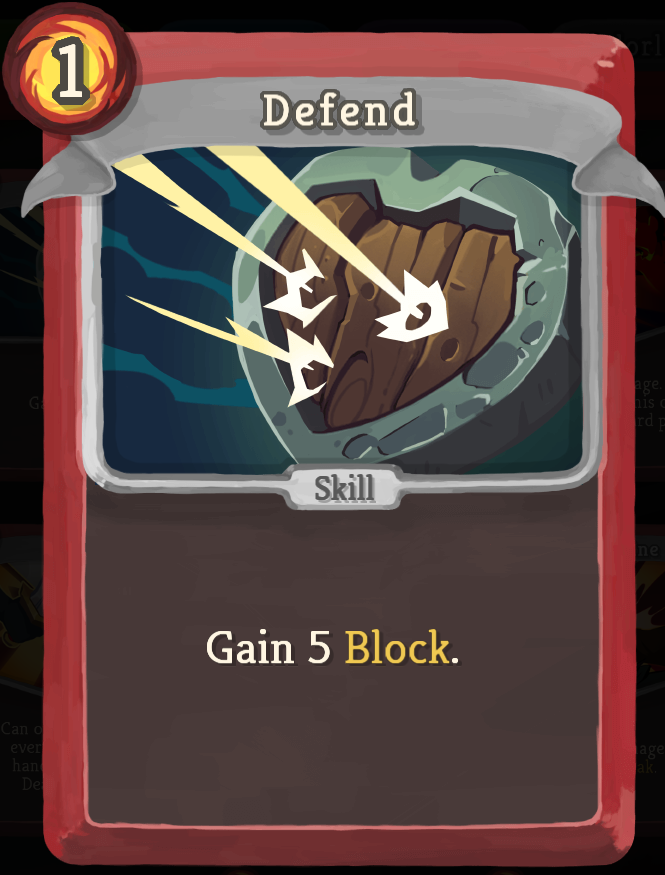
\includegraphics[width=0.95\textwidth]{img/Slay-the-Spire-Defend.png}
    \end{minipage}%
    \begin{minipage}{.25\textwidth}
        \centering
        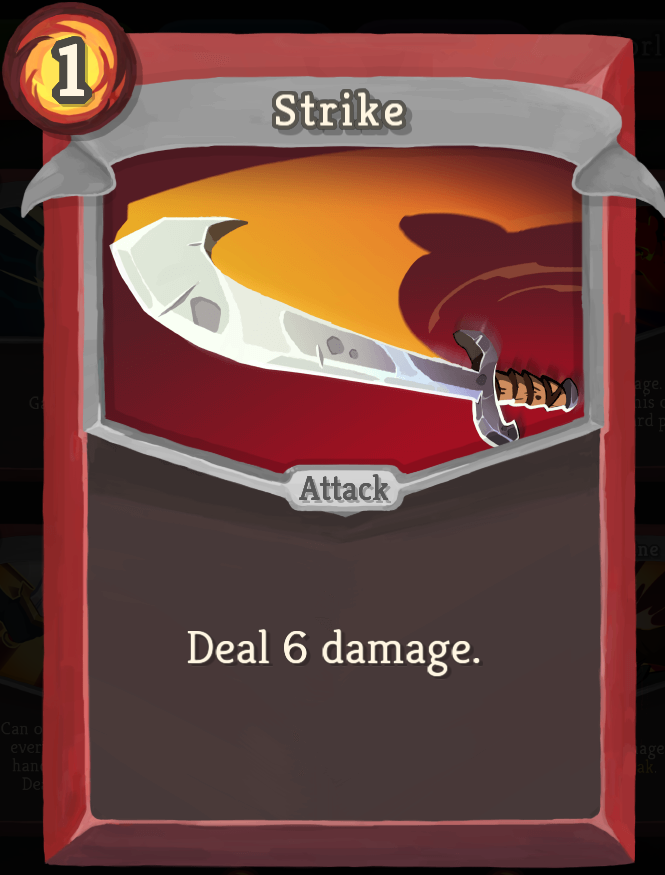
\includegraphics[width=0.95\textwidth]{img/Slay-the-Spire-Strike.png}
    \end{minipage}%
    \begin{minipage}{.25\textwidth}
        \centering
        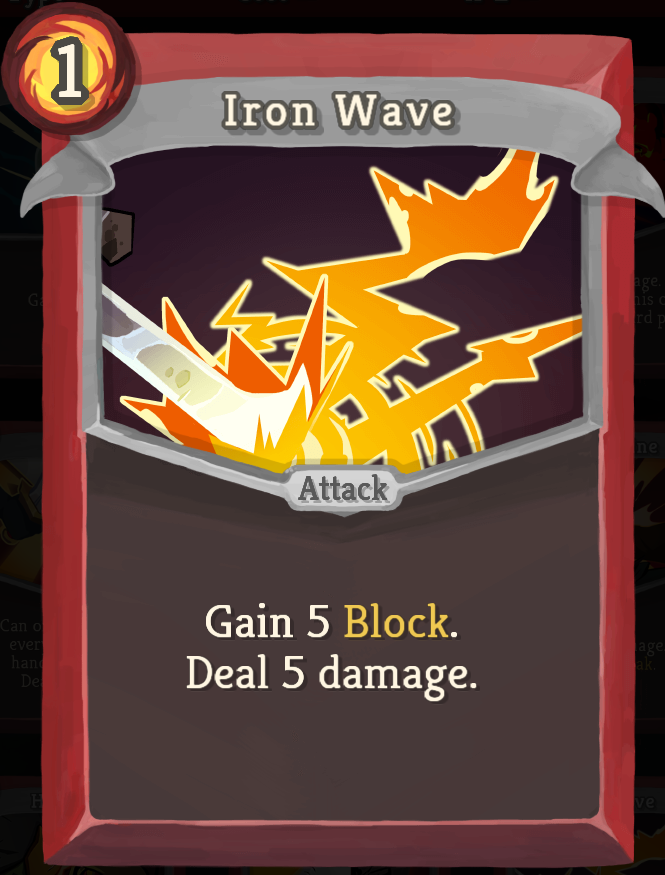
\includegraphics[width=0.95\textwidth]{img/Slay-the-Spire-Iron-Wave.png}
    \end{minipage}%
    \begin{minipage}{.25\textwidth}
        \centering
        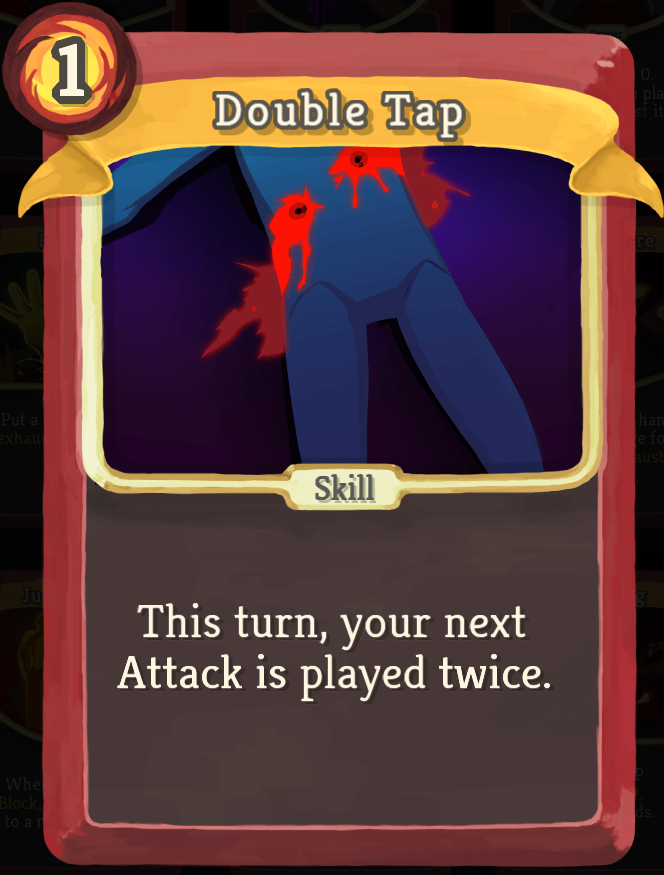
\includegraphics[width=0.95\textwidth]{img/Slay-the-Spire-Double-Tap.png}
    \end{minipage}
    \caption{\emph{Defend}, \emph{Strike}, \emph{Iron Wave} and \emph{Double Tap} cards from \emph{Slay the Spire}.}
    \label{fig:sts-iron-wave-and-double-tap}
\end{center}

We can design the blueprints in our game similarly, making some useful early in the run and some powerful later.
This will let the player decide if they need to take a blueprint that will help them now, or a blueprint that can potentially be strong later.

\subsection{Make Various Builds Viable} \label{sec:goal-various-builds}

One of the goals of our game is that the player should be able to beat the game with a lot of different combinations of blueprints.
We will call these combinations \emph{builds}, as is often done~\cite{buildDict} for unique combinations of skills, attributes and items a player's character can have in a role-playing game.
Builds are distinguished mainly by what they feel like to play with.
If two blueprints are used in the same way, then exchanging one for the other doesn't make a new build.
To allow the player to choose from various builds, there has to be enough blueprints that feel distinct and better yet, they should interact with other blueprints in unique ways.

In figure \ref{fig:pvz-almanac} are shown all the plants from \emph{Plants vs.\ Zombies}.
As we can see, there is a lot of them, and various combinations that work well are possible.
The plants usually don't interact with each other strongly, so the player mostly has to combine the plants such that they have no weak spots.
For example, longer levels require both cheap and expensive defensive plants.
The cheap plants are used at the start of the level, and later they are replaced by the more expensive ones to fit more firepower on the limited lawn.
Some plants can struggle against certain zombie types, so the player also wants to choose plants to cover for all their weaknesses.

\begin{center}
    \captionsetup{type=figure}
    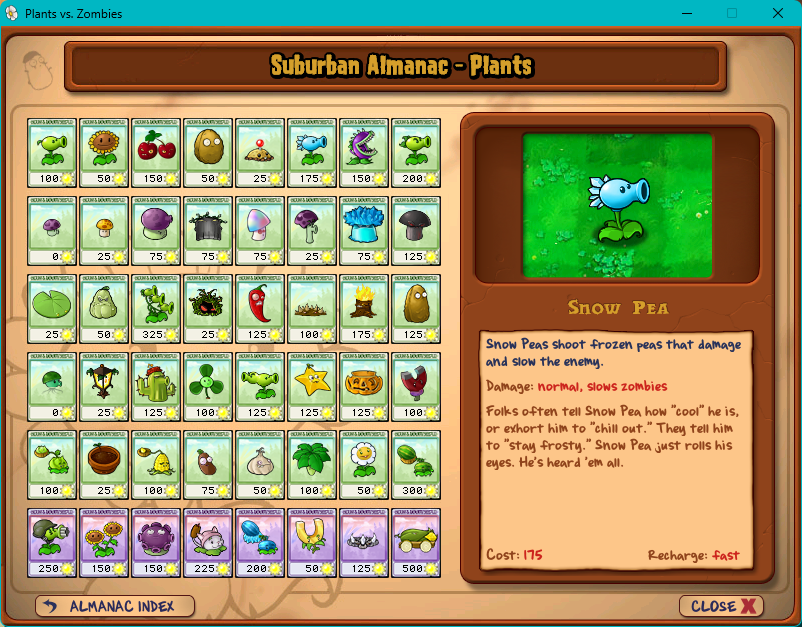
\includegraphics[width=0.8\textwidth]{img/Plants-vs-Zombies-Almanac.png}
    \caption{All the plants of \emph{Plants vs.\ Zombies} in the in-game almanac.}
    \label{fig:pvz-almanac}
\end{center}

We can also look at a few examples from \emph{Slay the Spire}.
Here, builds are often defined by cards that interact in ways that make them stronger.
One of the most blatant examples are cards that apply \emph{poison} to the enemy.
A poisoned enemy takes damage every turn based on the amount of \emph{poison} they have, and the amount decreases by one every turn.
This means an enemy with 2\,\emph{poison} takes $2 + 1 = 3$ damage in total, whereas an enemy with 4\,\emph{poison} takes $4 + 3 + 2 + 1 = 10$ damage in total.
It's easy to see that every card that applies \emph{poison} makes other \emph{poison} cards stronger.

There are also rare cards the player can find, which change how the game works.
For example, defensive cards provide \emph{block} only for one turn because the player character loses all \emph{block} at the start of every turn.
However, once the player plays the card \emph{Barricade}, they don't lose block at the start of their turns for the rest of the fight.
Cards like this can determine the player's strategy for the rest of the game on their own.

We want the players of our game to try lots of different builds and for that, the builds need to be strong enough to beat the game when the player executes them well.
We can tweak the strength of individual blueprints, but we can also design enemies that punish specific builds that would otherwise be too good.
For example, in \emph{Slay the Spire}, many enemies shuffle unplayable cards into the players deck for the duration of the fight.
This punishes decks with fewer cards way more than decks with many cards, keeping small deck builds from being too powerful.

\subsection{Force Exploration} \label{sec:goal-force-exploration}

We don't want the player to just find a single build that works and never explore anything new.
When the player is familiar with a build, it becomes stronger, since they know how to use it effectively.
This discourages them from trying other builds, because they can't use them so well, making them weaker.
Thus, one of our goals is to force the player to explore and make them learn other strategies.

The main way to get cards in \emph{Slay the Spire} are the rewards after every battle, where the player can choose one of three cards to add to their deck, as shown in figure \ref{fig:sts-card-reward}.
All the ways to acquire cards are randomized, so the player can't just hope to always get the card they want.
They have to adapt their build to the cards on offer, so they have to explore different strategies in order to win consistently.
In our game, the player will also pick a blueprint to add to their collection from a randomized offer after each battle.

\begin{center}
    \captionsetup{type=figure}
    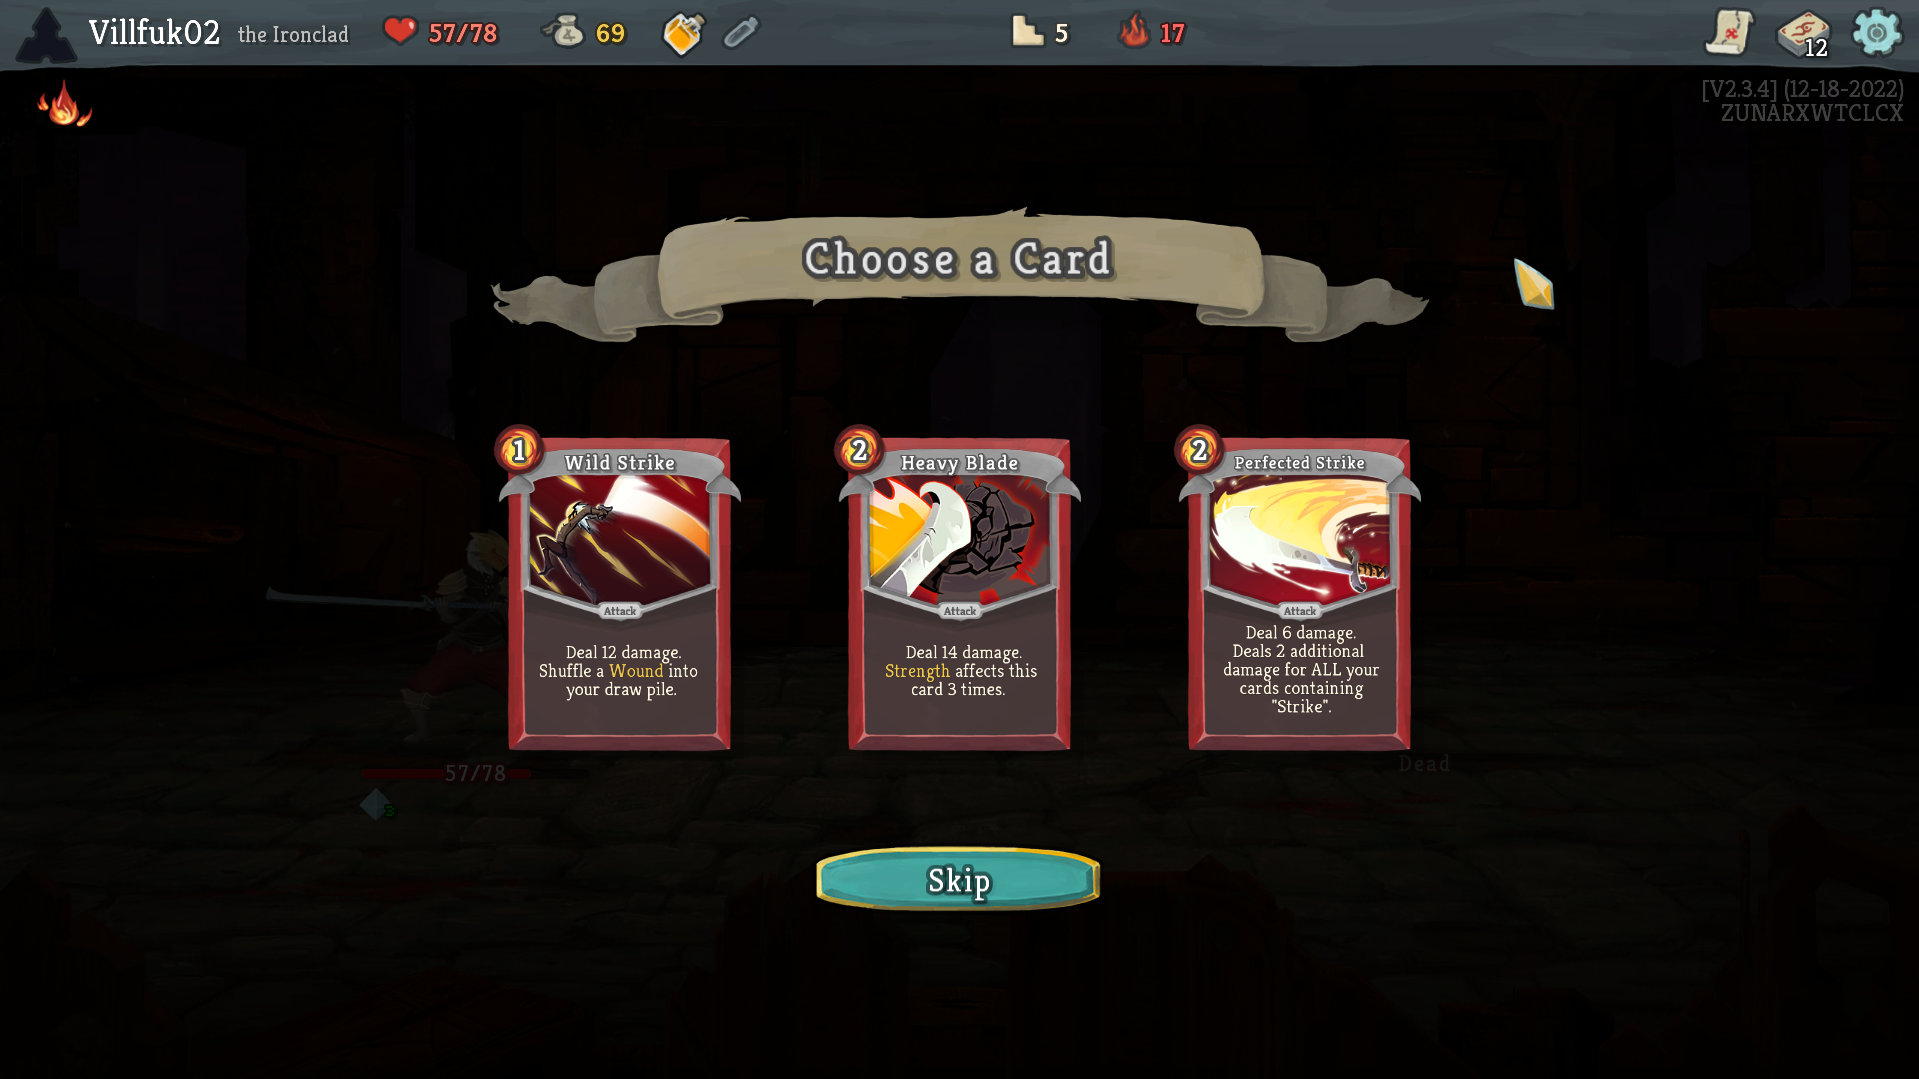
\includegraphics[width=0.8\textwidth]{img/Slay-the-Spire-Reward.png}
    \caption{Card reward screen in \emph{Slay the Spire}.}
    \label{fig:sts-card-reward}
\end{center}

In \emph{Plants vs.\ Zombies}, the player has to adapt to different zombies and level environments.
This can be illustrated with figure \ref{fig:pvz-roof}, which shows a seed select screen.
Here, the player selects which plants they want to use in this level from the selection on the left side.
On the right the player can see that this level takes place on the roof and the zombie types that will appear in this level.
In rooftop levels, the player has to place a \emph{Flower Pot}, which costs 25\,\emph{sun}, on a tile before they can place a plant there.
Furthermore, all plants that shoot in a straight line are of little use here because the roof slopes up, so their projectiles can't travel very far.
An experienced player will also notice that \emph{Bungee Zombies} will appear.
These zombies swing from above to take the player's plants instead of coming from the right.
The player should consider all these factors when choosing the build to play this level with.

\begin{center}
    \captionsetup{type=figure}
    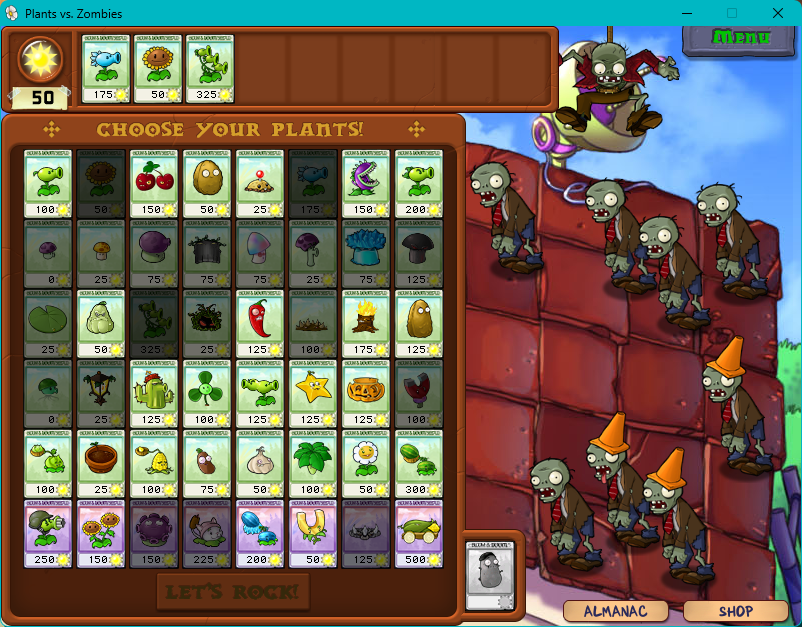
\includegraphics[width=0.8\textwidth]{img/Plants-vs-Zombies-Rooftop.png}
    \caption{Seed select screen in a rooftop level in \emph{Plants vs.\ Zombies}.}
    \label{fig:pvz-roof}
\end{center}

In our game, the player could select which blueprints to play with before every battle based on the level's features and attackers.
Instead, we chose an approach more similar to \emph{Slay the Spire}~--- the player will keep the blueprints they collect for the rest of the run, and they won't know the specifics of a battle before selecting it.
However, they will be allowed to have only a limited amount of blueprints at once, so they still cannot just keep all the blueprints they encounter.

\subsection{Provide a Challenge} \label{sec:goal-challenge}

The player should always have some goal to work towards, just out of their reach.
If the game is too easy, the players will have no reason to think strategically or learn.
Always having a harder challenge to overcome will motivate the player to improve and keep playing.

\emph{Slay the Spire} is not easy to beat, but the player can still improve so much even after beating the game.
After beating the game, the player unlocks so-called \emph{ascension}.
Before embarking on another run, the player can select the \emph{ascension} level they want to play on.
Each level introduces a small change that makes the game slightly more difficult.
Each \emph{ascension} level is unlocked only after the previous level is beaten, and each difficulty increase is small, so it doesn't discourage the player.
These changes are cumulative, so in the end it takes serious effort and luck to beat the game on \emph{ascension} level~20 even for the most skilled players.

\begin{notindemo}
    This system is simple, yet effective, so we might as well use it too.
    We will also want to balance the base game, so that most players that try are able to beat it, but it still takes some effort and several attempts, so the players feel like they've accomplished something.
\end{notindemo}

\section{Procedural Generation}

Randomized procedural generation is one of the defining features of the roguelike genre.
We want to use randomized procedural generation to make each run of the game unique.
Since we design the procedural generation algorithms ourselves, we have great control over the results.
However, procedurally generated parts of the game can be really hard to balance.
We need to make sure the randomized parts of the game feel fair to the player.
It doesn't feel good if the player loses the game because they were just unlucky and couldn't have done anything to prevent the loss.
Another issue with randomized procedural generation is that things might start to feel very homogenous.
For example, hand-crafted levels can have features that really stand out.
We need to decide which parts of our game will be procedurally generated and to what degree.

\begin{notindemo}
    The overall structure of each run will be decided by what we call the \emph{map}.
    As stated before, it will be a graph, and the player will go from node to node along the edges.
    Each node will be a battle, shop or an event.
    We really want each run to be different enough, that the player doesn't develop a single strategy to use in every run.
    Since the player will decide where to go, it's not a problem when some paths through the map are more difficult than others.
\end{notindemo}

Every battle will also be randomized to a large degree.
The world a battle takes place on will be procedurally generated, making for a different environment every time.
However, the combination of features that can appear in a given world will be decided by the world's \emph{terrain type}.
\begin{notindemo}
    There will be several hand-crafted terrain types to randomly select from, some appearing only early in the run and some only later.
    This is to create several cohesive styles of the worlds that look and play distinctly from each other.
    We feel this is better than if we just let the world generator mix all the features every time, because the results would be more homogenous.
    We will go into more detail about the world generation and these features in section~\ref{sec:design-world}.
\end{notindemo}

In \emph{Slay the Spire}, each encounter is chosen from a pool of hand-picked enemy combinations.
Each of these pools contains encounters of similar difficulty.
If the authors of \emph{Slay the Spire} decide one of the encounters is too difficult for its pool, they can tweak the encounter to make it less difficult, or move it to a different encounter pool.

In our game, however, the attacker waves in each level will also be procedurally generated.
We want this, because each level in our game will consist of many waves, each with many attackers.
We could design many sets of waves, but we feel that would make the levels too predictable, once a player learns these sets.
So, the waves shouldn't be tied to the previous waves in a level.
Each wave in a level will be harder and harder, so this would mean we would have to populate tens of pools with hand-crafted waves, which feels very inefficient.

We could also procedurally generate the blueprints and attacker types.
However, here we want to have greater control, because that will allow us to create designs that have powerful and unique abilities.
Procedurally generating these would be very difficult, and it would often lead to abilities that are either uninteresting, or way too powerful.

\section{Battle}

As stated in section~\ref{sec:original-vision}, in our game, the player will fight in battles throughout each run, and these battles will have tower defense gameplay.
In this section, we will describe the battles in more detail and explain our intentions.

\subsection{Attacker Waves}\label{sec:design-attacker-waves}

The attackers in various tower defense games often come in waves.
However, in \emph{Plants vs.\ Zombies}, the zombies also come in continuously throughout a level in addition to the large waves, to keep the pressure up.
Even in games where attackers come in distinct waves, the waves are usually on a timer and once the level starts, they keep coming.
One example of such a game is \emph{Kingdom Rush}~\cite{kingdomRush}.
In figure~\ref{fig:kr-next-wave} is shown the indicator which shows the time remaining to the next wave.
This means the game is also full of action and requires the player to think quickly.
Furthermore, this indicator lets the player call the next wave early.
If they do, they get some coins as a reward, but this is risky, because the player's defense might get overwhelmed.

\begin{center}
    \captionsetup{type=figure}
    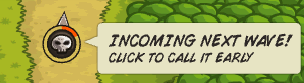
\includegraphics[width=0.6\textwidth]{img/Kingdom-Rush-Next-Wave-Detail.png}
    \caption{Next wave indicator from \emph{Kingdom Rush}.}
    \label{fig:kr-next-wave}
\end{center}

However, we want to emphasize the long-term strategy, so we will give the player plenty of time to plan out their next move.
There won't be any timer, instead, they can start the next wave when they are ready.
This is also common in tower defense games, used for example by \emph{Bloons TD 6}~\cite{BTD6}.
This brings our game closer to the turn-based gameplay that is often featured in roguelike games.
First it is the player's turn to build towers, and then the attackers' turn.

There are also many ways the attackers can move in different tower defense games.
Most often, the attacker paths are predetermined, and the player builds their towers around them.
The attackers go from the start of the path and try to reach the end of the path.
This is especially great when there is multiple different levels in the game, each featuring different paths, because it makes different towers more useful than others in each level.
In figure \ref{fig:btd6-maps} are shown two levels with distinct paths from \emph{Bloons TD 6}.
The path in the first level shown has a lot of tight turns, perfect for close-range towers or towers which damage all attackers in an area.
In the second level, the path is made up of few long straight segments, where are much more useful towers that pierce through many attackers in a straight line.
Since we want to have various procedurally generated levels in our game, we will also have attackers come on predefined paths that will be different in each level.

\begin{center}
    \captionsetup{type=figure}
    \begin{minipage}{.5\textwidth}
        \centering
        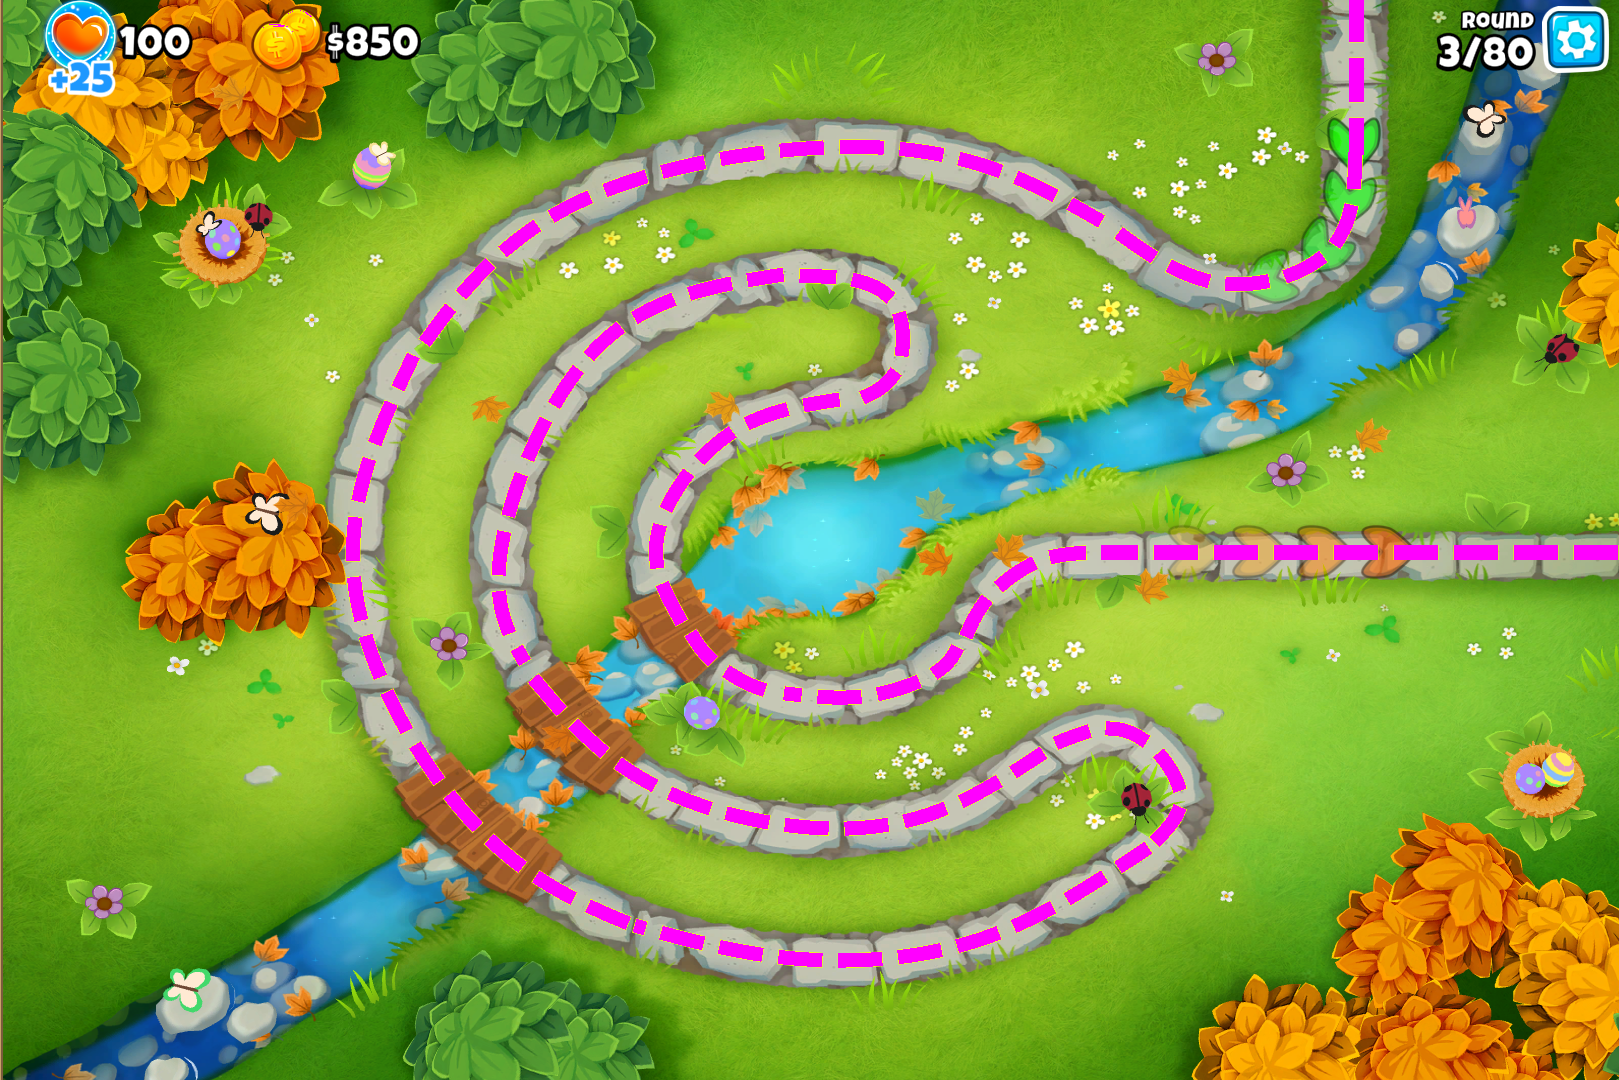
\includegraphics[width=0.95\textwidth]{img/Bloons-TD6-Park-Path-Highlighted.png}
    \end{minipage}%
    \begin{minipage}{.5\textwidth}
        \centering
        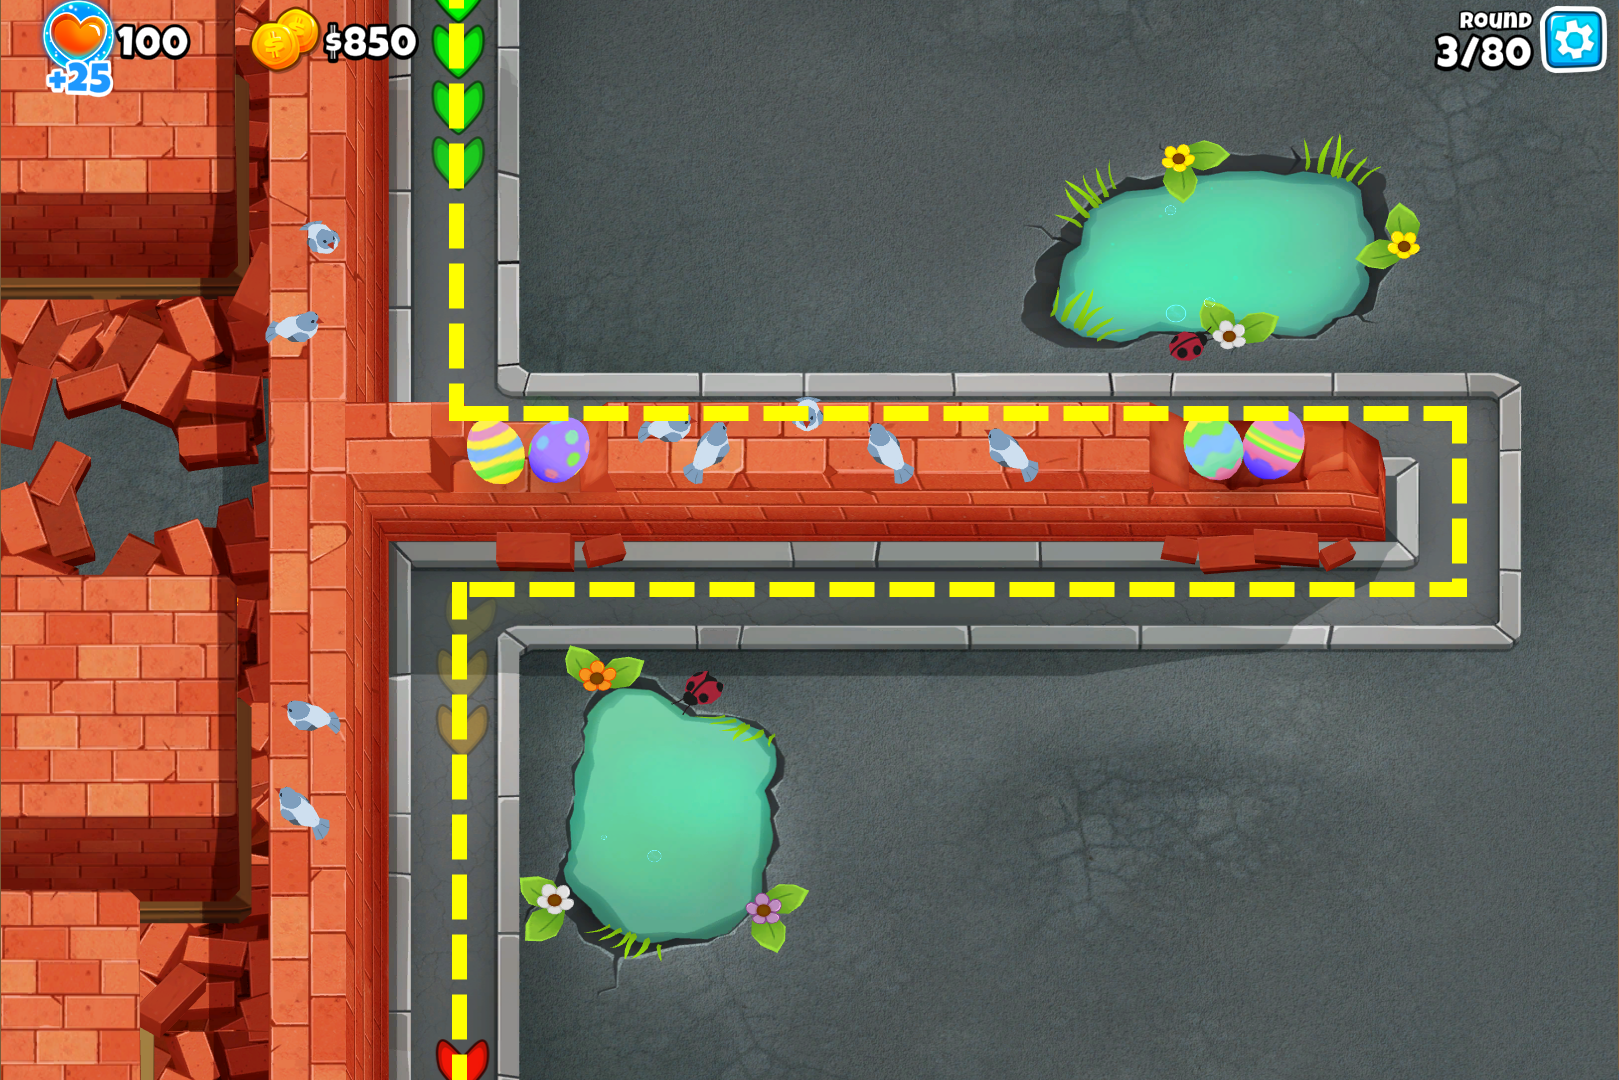
\includegraphics[width=0.95\textwidth]{img/Bloons-TD6-Another-Brick-Highlighted.png}
    \end{minipage}
    \caption{The levels \emph{Park Path} and \emph{Another Brick} from \emph{Bloons TD 6} with the attacker paths highlighted.}
    \label{fig:btd6-maps}
\end{center}

There are other options used in other games.
In \emph{Desktop Tower Defense}~\cite{DTDWiki}, for example, the attackers try to cross a rectangular playing field.
It starts out empty, but as the player fills it with towers, the attackers have to adjust their path, because they cannot go through the towers.
In figure~\ref{fig:dtd-pathfinding}, we can see the purple attackers funnel into a narrow passage between the white towers.
Since the player decides the path of the attackers, they have to learn what kind of path works well, but then they can build it all the time.
This is not ideal for us, because we want the player to adapt to the environment, not the other way around.

\begin{center}
    \captionsetup{type=figure}
    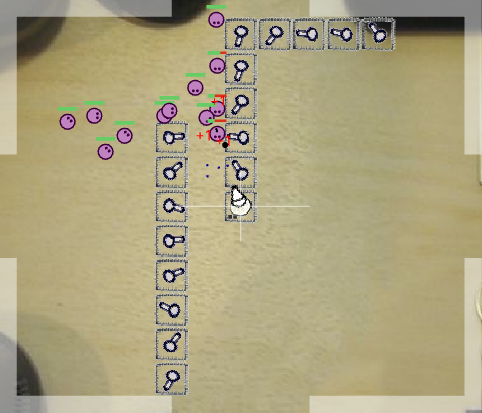
\includegraphics[width=0.6\textwidth]{img/Desktop-Tower-Defense-Playfield.png}
    \caption{Attackers being funneled between towers in \emph{Desktop Tower Defense}.}
    \label{fig:dtd-pathfinding}
\end{center}

In \emph{Plants vs.\ Zombies}, the zombies come from the right side of the screen and try to reach the left side, as we already mentioned.
The plants are planted directly in the way of the zombies and the zombies have to eat their way through them to reach their goal.
This is unique, and it greatly changes the gameplay.
However, this is again not great for our game, because we would lose a lot of potential for the levels in our game to be distinct from each other.

In \emph{Bloons TD 6}, the player receives very little information about what the upcoming waves look like.
Here, the player selects the level they want to play on, but the same sequence of waves comes every time, so the player is expected to learn at least those waves that give them problems.
In our game, however, the waves will be procedurally generated.
We want the player to plan around the upcoming waves, so we need to communicate what the upcoming waves are going to be.
This means that the waves should be simple enough to communicate effectively.
\emph{Desktop Tower Defense} features a wave preview, shown in figure~\ref{fig:dtd-waves}, that only describes the type of attacker that will come.
We want interesting behavior to emerge from the interaction of different attacker types, so we won't limit our waves to one attacker type, but instead three.
We feel that any more would make the waves messy and unnecessarily hard to communicate.

\begin{center}
    \captionsetup{type=figure}
    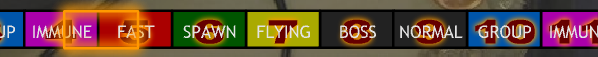
\includegraphics[width=0.8\textwidth]{img/Desktop-Tower-Defense-Waves.png}
    \caption{Wave preview from \emph{Desktop Tower Defense}.}
    \label{fig:dtd-waves}
\end{center}

In fact, each wave will be composed of one to three \emph{batches}.
Each batch will be composed of a number of attackers of only one type, spaced evenly.
But some waves will be just one batch, but this batch will send a different attacker type on each path on levels with multiple paths.
This should provide enough variety without being too hard to communicate to the player and too hard for a skilled player to predict the wave difficulty.

The waves in a single battle will get progressively harder, forcing the player will to improve their defense.
However, the wave difficulty should increase faster than the player's defense is expected to improve.
This increase will need to be carefully balanced to allow for some strategies where the player invests more into \emph{fuel} production to end a battle quickly, but also strategies where the player invests heavily into defense to keep up with the later waves.

\subsection{World}\label{sec:design-world}

In some tower defense games, for example in \emph{Desktop Tower Defense}, the towers can only be placed in positions on a grid.
In other games, for example \emph{Bloons TD 6}, the towers can be positioned freely, as long as they don't collide with each other, the attacker paths, or other obstacles.
While the second option might allow for more interesting tower placement, we will go with grid placement, and the grid will be pretty coarse~--- only $15 \times 15$ tiles.
In fact, the attacker paths will also be restricted to the grid.
They will be formed by segments, each going from the center of one tile to the center of a neighboring tile.
This is because we want the experience a player gains in one level to be transferrable to another level.
For example, they might learn that \enquote{tower A} placed right next to a straight path can handle a wave of five \enquote{attackers B} on its own.
They will then know this is true in any level whenever there is a sufficiently long straight path.
Reducing the number of path shape and tower position combinations will make the player come across a combination they already know more often, letting them predict better if their defense can handle a wave or not.
This is a really important skill to learn, because the player will have to decide before every wave, if they need to invest into defense or if they can invest into their economy.

In some tower defense games, for example in \emph{Kingdom Rush}, there are only few places where the player can place a tower in each level.
We feel this is too restrictive for our game, and it would take too much freedom away from the player.
This option also really works only in hand-crafted levels, because it is important to select the places for the towers in a way that makes for fun and interesting levels.

However, each level being just a big square of tiles with rectilinear paths on top wouldn't be very interesting.
That's why some tiles will contain obstacles that block the player from building on these tiles.
Some obstacles will be \emph{small} and some will be \emph{large}~--- they will also block the line-of-sight of towers that require a straight line between them and the attacker they want to shoot.
Some small obstacles will make the tile rich in \emph{minerals} (see section~\ref{sec:design-materials-and-energy}) or \emph{fuel} (see~\ref{sec:design-fuel}).
These will be used by some economic buildings (see~\ref{sec:design-buildings}), and also act as \emph{small} obstacles.

Another great way to make the levels more interesting, that is also intuitive for the player, is having tiles at different heights.
The heights will be in multiples of $0.5$ units, where one unit is the edge length of a tile.
Towers that require line of sight won't be able to shoot over higher terrain or down from steep cliffs.
We can also make some tower unable to shoot uphill or downhill for more variety.
Some tiles will also be slanted, gradually going from one height to another.
These tiles will allow the attacker paths to change their height, because it would be weird if the attackers had to jump up a cliff.
Some buildings will be possible to build on slanted tiles and some won't, making slants also a kind of obstacle.

As we already mentioned, each level will randomly select one of multiple \emph{terrain types}.
A terrain type will dictate how a terrain should look~--- the colors used, which terrain feature will appear and how often, and which obstacles will appear.
Each terrain type will have its distinct look, keeping the levels from being all the same.

To summarize:
\begin{itemize}
    \item The world each level takes place on will be a grid of $15 \times 15$ square tiles.
    \item There will be \emph{small} or \emph{large} obstacles on some tiles, large obstacles blocking certain towers' line of sight.
    \item The tiles will be at different heights in multiples of $0.5$ units, and some tiles will be slanted, going between two heights.
    \item Attacker paths will consist of segments going from the center of one tile to the center of a neighboring tile.
    \item The player can build one building per tile, and only if the tile doesn't contain an obstacle or the attacker path.
    \item Each world will be generated according to a randomly selected terrain type, which determines what the world will be like.
\end{itemize}

\subsection{Attacker Paths}\label{sec:design-paths}

In section~\ref{sec:design-attacker-waves} we decided that the attackers will travel on predefined paths generated with the world.
If we designed each level of our game by hand, we could create paths that just feel like they would be fun to play around.
Since the paths will also be procedurally generated, we need to describe what qualities should the paths have, so the generation can later be implemented to produce such paths.

In the previous section~\ref{sec:design-world} we decided that the world will consist of a grid of tiles and the paths will be constrained to straight segments between the centers of the tiles.
We can think of the paths segments as one-way passages between neighboring tiles.
This means that a path cannot go twice through the same tile or cross itself, because a tile has the same path segments coming from it, no matter if it was visited for the first or second time.

There can be multiple paths in a level, each with a different shape and in some waves a different set of attackers.
This will add more variety and depth to tower placement.
Any path will also be able to split into more paths, or join together with another path, creating new path geometry or sections with different attacker density.
When a line of attackers comes to a split into multiple paths, they will alternate in which path they continue to, splitting between the paths evenly.

The player will start each level with one building already built~--- the \emph{Hub}.
It is the goal the attackers are trying to reach to destroy it.
Hence, all attacker paths will converge to the tile the Hub is on.
The attackers will come from outside the world the battle takes place on.
In the game's universe, the worlds are bigger, but the playable area is just a small neighborhood around the Hub.
It would be weird if the attackers just appeared on the edge tiles, so their paths will start on tiles just outside the playable world.

In figure~\ref{fig:valid-path-example} we can see an example of a valid path network drawn in blue on a world of square tiles.
The black point represents the Hub.

\begin{center}
    \captionsetup{type=figure}
    \begin{tikzpicture}
        \draw[step=1.0,black,thin] (0,0) grid (7,7);
        \begin{scope}[blue,very thick,decoration={
                        markings,
                        mark=between positions 0.25cm and -0.15cm step 0.5cm with {\arrow{>}};
                    }]
            \draw[postaction={decorate},shift={(0.5,0.5)}] (-1,1)--(1,1)--(1,5)--(3,5)--(3,4)--(5,4);
            \draw[postaction={decorate},shift={(0.5,0.5)}] (1,2)--(3,2)--(3,1)--(5,1)--(5,4);
            \draw[postaction={decorate},shift={(0.5,0.5)}] (3,-1)--(3,1);
        \end{scope}
        \filldraw[black] (5.5,4.5) circle (5pt);
    \end{tikzpicture}
    \caption{An example of a valid path network in a $7 \times 7$ game world.}
    \label{fig:valid-path-example}
\end{center}

The attackers from single wave batch will start out evenly spaced.
If the path they are on splits into two, they will still be evenly spaced, but now the spacing is twice as large.
This is illustrated in figure~\ref{fig:attackers-path-split}, where the attackers are represented by black dots on the path.
We can also see, that after the paths join back into one, the attacker spacing is no longer even.
We don't want this to happen for aesthetic reasons, but also because overlapping attackers could be hard to identify or distinguish by the player.
This only happens when the branches of a path are of unequal length and the difference is not a multiple of the spacing between the attackers.
We don't want to put more constraints on attacker spacing, so instead, we will constrain path branches to be of equal length.
More precisely, each tile on a path has to be the same distance from the Hub, no matter which path an attacker would take.

\begin{center}
    \captionsetup{type=figure}
    \begin{tikzpicture}
        \begin{scope}[blue,very thick,decoration={
                        markings,
                        mark=between positions 0.25cm and -0.01cm step 0.5cm with {\arrow{>}};
                    }]
            \draw[postaction={decorate},shift={(0.5,0.5)}] (-1,1)--(2,1)--(2,2)--(4,2)--(4,1)--(8,1);
            \draw[postaction={decorate},shift={(0.5,0.5)}] (2,1)--(4,1);
        \end{scope}
        \filldraw (-0.3,1.5) circle (3pt);
        \filldraw (0.9,1.5) circle (3pt);
        \filldraw (2.1,1.5) circle (3pt);
        \filldraw (3.3,1.5) circle (3pt);
        \filldraw (4.5,1.5) circle (3pt);
        \filldraw (5.7,1.5) circle (3pt);
        \filldraw (6.9,1.5) circle (3pt);
        \filldraw (8.1,1.5) circle (3pt);
        \filldraw (0.3,1.5) circle (3pt);
        \filldraw (1.5,1.5) circle (3pt);
        \filldraw (2.5,1.7) circle (3pt);
        \filldraw (2.9,2.5) circle (3pt);
        \filldraw (4.1,2.5) circle (3pt);
        \filldraw (4.5,1.7) circle (3pt);
        \filldraw (5.5,1.5) circle (3pt);
        \filldraw (6.7,1.5) circle (3pt);
        \filldraw (7.9,1.5) circle (3pt);
    \end{tikzpicture}
    \caption{Attackers on a path that splits and joins.}
    \label{fig:attackers-path-split}
\end{center}

Most towers will have limited range, and they will be most effective near the attacker paths.
We want the paths to be spread out throughout the game world in order to not have tiles that are just way too far from any paths to be useful.
This is illustrated in figure~\ref{fig:path-spacing}, where we can see a path network with bad features on the left, and on the right, one with the same path lengths and starting positions, but nicer and more spread out.
We have marked tiles whose center is 2 or more tiles from the nearest path with a small cross.

In the right figure, we can also see a red point on one tile, marking a great spot for a tower.
This spot allows even a tower with shorter range, illustrated by the red ring around it, to target attackers on a large portion of the path.
On the left we have circled another U-turn in the path that is, however, undesirable.
This is because there is no empty tile between the paths, so the player can't place a tower there, which feels bad.
We don't want many sharp turns like these, but they can occur from time to time for variety.
Similarly, paths going right next to each other (marked in red) are bad.
The player cannot place towers on paths, so these paths greatly limit the player's access to each other, making for an unpleasant experience.
A similar situation occurs when a path goes through tiles at the edge of the world, blocking access to the path from one side, so paths should not go through these tiles very often.

The Hub should be several tiles away from the edges of the playable area, so the player has good access to the path segments near it.
It should be very close to the center in levels with many paths, so the paths can come towards it from different sides of the world.
It can be more off-center in levels with only one or two long paths, where the path can snake through the world from the side furthest away from the Hub, also covering the world somewhat evenly.

\begin{center}
    \captionsetup{type=figure}
    \begin{tikzpicture}
        \draw[step=1.0,black,thin] (0,0) grid (6,6);
        \draw[step=1.0,black,thin] (7,0) grid (13,6);
        \begin{scope}[blue,very thick,decoration={
                        markings,
                        mark=between positions 0.25cm and -0.15cm step 0.5cm with {\arrow{>}};
                    }]
            \draw[postaction={decorate},shift={(0.5,0.5)}] (2,6)--(2,5)--(1,5)--(1,4)--(4,4);
            \draw[postaction={decorate},shift={(0.5,0.5)}] (5,6)--(5,4);
            \draw[red,postaction={decorate},shift={(0.5,0.5)}] (4,4)--(4,1);
            \draw[red,postaction={decorate},shift={(0.5,0.5)}] (5,4)--(5,1);
            \draw[postaction={decorate},shift={(0.5,0.5)}] (5,1)--(3,1);
            \draw[postaction={decorate},shift={(0.5,0.5)}] (9,6)--(9,4)--(7,4)--(7,2)--(9,2)--(9,1)--(10,1);
            \draw[postaction={decorate},shift={(0.5,0.5)}] (12,6)--(12,3)--(11,3)--(11,1)--(10,1);
        \end{scope}
        \filldraw[black] (3.5,1.5) circle (5pt);
        \filldraw[black] (10.5,1.5) circle (5pt);
        \draw (0.5, 0.5) node[cross=2.5pt] {};
        \draw (0.5, 1.5) node[cross=2.5pt] {};
        \draw (0.5, 2.5) node[cross=2.5pt] {};
        \draw (1.5, 0.5) node[cross=2.5pt] {};
        \draw (1.5, 1.5) node[cross=2.5pt] {};
        \draw (1.5, 2.5) node[cross=2.5pt] {};
        \draw[red] (2,5) circle (0.8cm);
        \filldraw[red] (8.5,3.5) circle (4pt);
        \draw[red] (8.5,3.5) circle (1.6cm);
    \end{tikzpicture}
    \caption{A path network with undesirable properties and a path network with great properties.}
    \label{fig:path-spacing}
\end{center}

Similarly, we don't want to produce side branches that just take up more space, but don't deviate meaningfully from the original path, like on figure \ref{fig:bad-path-splits}.
To make this desire into a rule, we can define it in the following way:
Every side branch must go through at least one tile that is not adjacent (by an edge or by a corner) to any already existing path.

\begin{center}
    \captionsetup{type=figure}
    \begin{tikzpicture}
        \begin{scope}[blue,very thick,decoration={
                        markings,
                        mark=between positions 0.25cm and -0.01cm step 0.5cm with {\arrow{>}};
                    }]
            \draw[postaction={decorate},shift={(0.5,0.5)}] (0,2)--(2,2)--(2,1)--(7,1)--(7,2)--(8,2)--(8,1)--(9,1)--(9,2)--(10,2);
            \draw[postaction={decorate},shift={(0.5,0.5)}] (1,2)--(1,1)--(2,1);
            \draw[postaction={decorate},shift={(0.5,0.5)}] (3,1)--(3,2)--(7,2);
            \draw[postaction={decorate},shift={(0.5,0.5)}] (8,2)--(8,3)--(9,3)--(9,2);
        \end{scope}
    \end{tikzpicture}
    \caption{A path with undesirable side branches.}
    \label{fig:bad-path-splits}
\end{center}

To summarize, these are the rules the paths should follow:
\begin{itemize}
    \item Paths are formed by one-way segments, each from one tile to its neighbor.
    \item Paths start just outside the playable portion of the world, and there can be one or more path starts in each level.
    \item Paths can split or join.
    \item All paths must end on the tile with the Hub, no other dead ends can exist.
    \item Each tile with a path going through it has to be the same distance from the Hub no matter which path an attacker would take.
    \item Paths should be spread throughout the playable world, not bunched up.
    \item Paths right next to each other or the edge of the world, and sharp U-turns (see figure~\ref{fig:path-spacing}), should be rare.
    \item Every side branch must go through at least one tile that is not adjacent to any already existing path.
\end{itemize}

\subsection{Attacker Types}\label{sec:attacker-types}

We have mentioned that there will be many attacker types in out game.
Each will be designed on its own, but they will be randomly combined to make attacker waves.
An attacker type defines the following properties of an attacker:
\begin{itemize}
    \item \textbf{Appearance}. Every attacker will be represented in a battle by its 3D model, corresponding animations and other visual effects. Every attacker type will also have an associated icon to display in the user interface.
    \item \textbf{Hit Points} or \textbf{HP} determine how much damage can an attacker take from the towers before it dies.
    \item \textbf{Movement speed} in tiles per second.
    \item \textbf{Size}~--- either \emph{small}, \emph{large} or \emph{boss}~--- determines how much \emph{hull} (see section~\ref{sec:design-hull}) the player loses when this attacker reaches the Hub. Also defines the height off the ground of the spot defensive towers target. More details below.
    \item \textbf{Abilities}. These can be \emph{passive} (for example \enquote{Immune to fire.}), \emph{repeating} (\enquote{Heals 5\,HP every two seconds.}), or \emph{reactive} (\enquote{Spawns \emph{attacker A} when killed.}).
\end{itemize}

The height of a target a tower shoots at is important~--- lower targets can easily hide behind a terrain feature or an obstacle.
We want some attackers to look bigger than others, and it would be weird if the towers shot at a lower portion of their model.
Larger attackers will have their targeting point higher.
To make things simple for the player, there are only two heights of the targeting point~--- \emph{small} at $0.15$ units above the ground and \emph{large} at $0.3$.

Whenever an attacker reaches the Hub, the player will lose some \emph{hull}.
The \emph{small} attackers will come in greater numbers than \emph{large} attackers.
To make the stakes more equal, \emph{small} attackers cost the player only 1~\emph{hull}, whereas the \emph{large} attackers cost 3~\emph{hull}.

\begin{notindemo}
    The player will encounter only few \emph{boss} attackers in every run.
    They will be the main attackers in special boss levels, which are spread throughout the run and cannot be avoided by the player.
    When a boss reaches the Hub, the player immediately loses the game.
    Each boss will bend the rules of the game a bit as one of their abilities, but most of them will have the same target height as \emph{large} attackers.
\end{notindemo}

\subsection{Buildings}\label{sec:design-buildings}

The player will be able to build buildings, but only between waves of attackers.
They will be able to build one building per tile, if the tile has no obstacles and an attacker path is not going through it.
Each building costs some amount of \emph{materials} to build.
The player will be able to delete a building at any time, mainly to make way for other buildings.

There are three building types defined by their primary function: \emph{towers}, \emph{economic} and \emph{special}.
Towers deal damage and kill attackers, and they are described in more detail in the next section.
Economic buildings produce resources, often at the end of every wave, just in time for the player to use them to build more buildings.
Some economic buildings produce resources at other times, often as a reaction to some other event, for example an attacker dying.

Special buildings are the buildings that don't fit in either category.
They have a unique ability that usually increases the effectiveness of other buildings.
One special building could make economic buildings produce more, another could increase your towers' range, yet another might slow attackers down.

One notable special building is the Hub, since the player starts each level with one for free, and they cannot build more.
The goal of the attackers is to reach the Hub, and when they do, the player loses some \emph{hull} (see section~\ref{sec:design-hull}).
Additionally, the Hub produces some amount of \emph{fuel}, \emph{materials} and \emph{energy} at the end of each wave.
These resources are further described in their respective sections.

\subsection{Towers}\label{sec:design-towers}

Towers are the buildings which deal damage to attackers in order to kill them.
There are many properties that distinguish towers from each other.
There is a lot of freedom to allow for many unique designs.
Combining towers with different properties is supposed to be a fun and interesting part of the game.

Towers usually shoot once per their \emph{shot interval}, but some towers can shoot multiple projectiles at once, others deal a certain amount of damage per second continuously.
They can usually only target attackers in a circular range around them.
However, some towers have an unlimited range, or their range is not circular.
Most towers instantly aim at their target, some take time to rotate around and others cannot rotate at all.
Some towers cannot aim upwards or downwards.
Most towers require line of sight to their target, but some don't.
Most towers fire projectiles in a straight line, but some don't fire projectiles, others fire projectiles that travel over obstacles along a ballistic arc.
Some towers can even miss their target.
With tower designs, the sky is the limit.

Whenever a tower has more attackers in its range, it will decide which one to target based on the tower's targeting priority.
The player will be able to select one of these priorities on most towers:
\begin{itemize}
    \item First~--- the attacker that's closest along its path to the Hub.
    \item Last~--- the attacker that's farthest along its path from the Hub.
    \item Closest~--- the attacker that's closest to this tower.
    \item Farthest~--- the attacker that's farthest from this tower.
    \item Weakest~--- the attacker with the least HP.
    \item Strongest~--- the attacker with the greatest HP.
\end{itemize}
Each tower will be set to one of these by default, but the player will be able to change the priority of any tower at any time, even during waves.
This will let the player have more control over their towers, allowing them to best use their unique properties.

The damage the towers deal comes in many types.
For example \emph{physical}, \emph{explosive}, \emph{energy}.
Some towers will deal damage of multiple types at once.
This distinction lets us make some towers explicitly weak against some attackers~--- those that are resistant to the given damage type.
Or it lets us restrict some synergies, for example by making a building that makes attackers take more damage from \emph{energy} attacks only.

It is worth mentioning, that in most tower defense games, the player can upgrade any tower during a battle by investing more resources into it.
The upgrades often increase a tower's damage or fire rate, however some substantially change the tower's behavior.
Some games take this to the extreme, for example in \emph{Bloons TD 6}, each tower has 15 different upgrades available, and each tower can be upgraded to two different upgrades at once.
However, in our game, the player won't be able to upgrade their towers during a battle.
Instead, they will have to have some towers that are useful at the start of a level, and others that are more powerful, but more expensive, to be used later.

\subsection{Abilities}\label{sec:design-abilities}

Unlike buildings, abilities will be usable during waves only.
They will often have only short-term effects on the attackers, so there is no point to using them outside a wave.
The primary use-case is to kill or weaken attackers of a wave that might be too difficult to deal with for the towers alone.
Abilities cost \emph{energy} to use, but if the \emph{energy} a player has is insufficient, \emph{materials} can be used to cover the difference.
The reasoning behind this is explained in the next section~\ref{sec:design-materials-and-energy}.

Most abilities will only deal damage to the attackers, each in its own unique way.
However, similarly to towers, there is no restriction on what an ability can do, as long as it makes gameplay sense and offers something new.
One ability could create a temporary defensive tower, another could temporarily improve the towers the player has already built.
Another ability might improve the player's blueprints for the rest of the battle, yet another might just give the player some additional resources.

\subsection{Materials and energy}\label{sec:design-materials-and-energy}

\textbf{Materials} are the main resource within a battle.
The player starts each battle with some materials, and the Hub produces a small amount of materials after every wave.
Materials accumulate over the battle and there is no limit as to how many the player can have.
The player can spend materials on buildings, notably towers and economic buildings.
The more economic buildings that produce materials a player builds, the more materials they will have later in the battle.

Intuitively, a great strategy is to build the towers necessary to survive the next wave and spend the rest on economic buildings.
However, this strategy heavily relies on the player being able to estimate which combination of towers is strong enough to beat the wave.
To help, the player will have various abilities at their disposal, which can be used to kill of or weaken attackers when the towers are not strong enough by a small margin.
The abilities should also cost resources to regulate their usage~--- stronger abilities will cost more and weaker abilities will cost less.
However, if abilities also cost materials, it would be the best to spend everything on permanent defense or economy.
Ideally a player would leave no materials for their abilities.
That is why abilities have a resource dedicated only to them~--- \textbf{energy}.
A steady income of energy lets the player use an ability once in a while, without costing them any long term power.

However, abilities can also be paid for in materials.
All this time we've assumed that long-term power is always better than short-term.
However, this is not necessarily true.
In the last few waves, a powerful one-time effect is way better than a weak long-term one, since the battle is ending soon anyway.
Due to this, abilities are perhaps most useful in the last few waves of a battle, and allowing the player to use materials for these lets them use the materials on whatever they think is the best.
Paying with materials also helps when the player has a few materials left over, so they can use a slightly more expensive ability than they could without this.

We don't want the player to hoard all their energy and only use it on the last waves.
To encourage using abilities throughout the battle, there will be a limit on the energy a player has in reserve.
This way there is much less downside to using an ability in the middle of a battle when the player's energy reserve is full anyway, so they can't get any more.

\subsection{Fuel}\label{sec:design-fuel}

We have already mentioned fuel a few times, for example in section~\ref{sec:original-vision} and section~\ref{sec:goal-depth-battle}.
But in this section, we will summarize everything about fuel.

The goal of each battle is to gather enough fuel to continue to the next level.
The faster the player gathers the fuel, the sooner they win the battle.
It is generated passively by the Hub, but additional buildings can be built to speed up the process.
This makes the player decide when it's the best to improve their defenses and when to build fuel-producing building instead, to end the battle before the more difficult waves come, hopefully leading to greater strategic depth.
The maximum number of waves each battle will take is determined by the amount of fuel the player needs to gather.

\begin{notindemo}
    We want some battles to be significantly harder, but they will provide better rewards.
    These will be marked on the map, so the player will decide if they want to risk a harder battle.
    Making these battles require more fuel to complete is a great way to distinguish them from other battles.
    This also applies to boss battles (see section~\ref{sec:attacker-types}).
\end{notindemo}

\subsection{Hull}\label{sec:design-hull}

The player starts each run with a fixed amount of hull.
As described in section~\ref{sec:attacker-types}, whenever an attacker reaches the Hub during a battle, the player loses some hull.
Once the player loses all hull, they lose the game.
A player's hull is a kind of buffer that allows them to make a few mistakes throughout the whole run before they lose.
They will be able to restore their hull only a few times during the run (and no hull can be restored in the demo version).
For example, they can intentionally focus more on economy in the early waves of a battle, maybe letting a few attackers through, in order to be stronger in the later waves and prevent possibly greater losses.
They can even take a harder battle where they expect to lose hull when they are confident they won't need it before they can restore it back.
However, an experienced player can use their hull as a resource.
Another option would be to have the player start each battle with full hull, but we feel that this option allows for way less strategic depth.

\subsection{Status Effects}

\begin{notindemo}
    Buildings and attackers will both be able to have status effects applied on them.
    These represent temporary effects which modify the behavior of whatever they affect.
    They will be displayed with an icon above what they are applied to, along with a number representing their duration.
    The duration can be measured in seconds, but other kinds of duration are possible.
    The source of these effects can be anything from a tower to an attacker.

    Here are few examples of effects that might be applied to attackers, $x$ representing their duration:
    \begin{itemize}
        \item \textbf{Burning} deals a small amount of \emph{energy} damage over time for $x$ seconds, possibly applied by some fire-based tower.
        \item \textbf{Freezing} slows down the attacker's movement speed for $x$ seconds, possibly applied by some ice-based ability.
        \item \textbf{Shield} prevents the next $x$ damage an attacker would take, possibly applied by another attacker.
        \item \textbf{Stealth} makes the attacker untargetable for the next $x$ seconds, possibly applied on their own.
    \end{itemize}

    And a few examples of effects that could be applied to buildings are:
    \begin{itemize}
        \item An \textbf{Overclocked} tower shoots 50\% faster for $x$ waves, possibly applied by an ability.
        \item A \textbf{Paralyzed} building is out of order for $x$ seconds, possibly applied by an attacker.
        \item The next $x$ projectiles an \textbf{Electrified} tower shoots deal additional \emph{energy} damage, possibly applied by a support building.
    \end{itemize}
\end{notindemo}

\subsection{Time controls}

\begin{notindemo}
    We want the player to be able to pause the game.
    This is a quality-of-life feature, common among other real-time single-player games.
    In our game, the waves are short, and the player can just not start the next wave until ready.
    However, pausing will be very useful during the waves for lining up ability placement.
    Some attackers move fast and hitting them can be difficult, and we don't want our game to focus on dexterity or reaction time.
    What's even more difficult is clicking on a fast moving attacker to inspect its details (described in section~\ref{sec:design-info-panel}).

    We will also let the player speed up the game to play at double speed.
    This is useful for less eventful portions of gameplay, for example when a slow-moving attacker travels along a long empty stretch of path.

    It is important that the game plays out the same no matter at which speed it's playing, and that pausing doesn't interfere with the game.
    For example, it would be bad if the towers sometimes missed their targets when playing at double speed.
    What happens in the game should also be frame rate independent.

    On the other hand, everything should look as smooth as possible given the frame rate at which is the game currently rendered.
    Some animations will have to speed up when the game speeds up, others will still play at the same speed, even when the game is paused.
\end{notindemo}

The demo version will be developed in a way that allows for this separation of game logic and game visuals.
However, the time controls themselves will not be available in the demo.

\section{Blueprints}\label{sec:design-blueprints}

A blueprint represents a building the player can build or an ability they can use during battles.
Each blueprint will include a description that explains its function, including the exact values of important statistics~--- for example the amount of damage a tower deals with each hit.
The player will start each run with few predefined blueprints, and they will collect more blueprints throughout the run, giving them access to more buildings and abilities.

The player will only be able to have a limited number of blueprints at any given time.
Whenever they want to acquire a new blueprint while at the limit, they'll have to give up one of the blueprints they already have.
This way it is impossible to make a build that is just good at everything.
They will have to consider carefully which blueprints they need to cover their weaknesses and which blueprints are the most synergistic with the rest.

Each blueprint costs some \emph{materials} and/or \emph{energy} (see section~\ref{sec:design-materials-and-energy}) to use, though there could be some blueprints that are free.
The player must pay this cost every time they want to build the given building or use the given ability.

Most blueprints will have no cooldown, so the player will be able to use them as of ten as they want.
Some will have a cooldown given as a number of waves.
This means some will be usable only once per wave, some only once per two waves, etc.

As we already mentioned a few times, the player will acquire new blueprints mainly after every battle.
The player will be presented with a selection of three different blueprints they have not picked in this run yet.
They can choose one of these to add to their collection, acquiring it for the rest of the run.
\begin{notindemo}
    Similar blueprint rewards will appear during some events the player might encounter.
    Some events will offer blueprints randomly selected from the same pool as battle card rewards, other events will offer predefined blueprints, which don't appear in the regular blueprint rewards.
    Some shops will also sell blueprints chosen randomly from the reward pool.
\end{notindemo}

In the regular blueprint rewards, some blueprints will be more rare than others.
Each blueprint will have one \emph{rarity}, which determines how often it will appear.
The rarities are
\begin{itemize}
    \item \textbf{common},
    \item \textbf{rare},
    \item and \textbf{legendary}.
    \item Additionally, there is \textbf{starter}~--- the player starts each run with these. Thus, they do not appear as rewards.
    \item And also \textbf{special}~--- these blueprints also do not appear in the regular blueprint rewards, but they can be obtained on other ways, usually in events.
\end{itemize}

As their name suggests, \emph{common} blueprints will be more common than \emph{rare} blueprints, and \emph{legendary} blueprints will be even more rare.
At first, the player will encounter a \emph{rare} blueprint about once per a few rewards with the rest being \emph{common}.
However, towards the end of the run, most blueprints on offer will be \emph{rare}.
Additionally, some rewards, for example after harder battles or boss battles (see section~\ref{sec:attacker-types}), will contain more rare blueprints more often.
The exact proportions are yet to be determined based on playtesting.

\subsection{Design}

The blueprints should be designed in such a way, that it is not great to always take the blueprint with the highest rarity.
Of course, rarer blueprints will usually be stronger, but they will usually be more specific in their use.
\emph{Rare} blueprints should be similarly good to \emph{common} blueprints in most cases, but potentially much stronger when used in the right way or in combination with the right blueprints.
\emph{Legendary} blueprints should have the greatest potential power, but in even more specific circumstances.
This power should however be so great, it is worth it to sacrifice some of the build's other aspects in order to get the most out of this blueprint.
The overall strategy of a given build could be defined by a few \emph{legendary} blueprints, with the rest built to support them.
Of course, some \emph{legendary} blueprints will be useful in more builds than others.
It should also be possible to make a strong build just with a good set of \emph{common} and \emph{rare} blueprints.

As we already mentioned in sections~\ref{sec:design-buildings}, \ref{sec:design-towers} and \ref{sec:design-abilities}, each blueprint should be unique in its own way.
The most exciting designs are often those that somehow break the rules.
For example, we could design a building that costs \emph{energy}, or a tower that has to be placed on a path, or even an ability that manipulates your blueprints or the waves of attackers that are yet to come.
However, most of these are hard to balance properly, and most important is whether they lead to fun gameplay or not.

It is also important to design a good set of starter blueprints.
It should be as small as possible, but somewhat balanced in most aspects.
Specifically, it should provide a way to gather \emph{materials} and \emph{fuel}.
There should be at least two towers that can deal with the early levels, and they are distinct from each other, so there are still decisions to make even in the first levels.
There should also be a starter ability, since abilities are a core of the design (see section~\ref{sec:design-abilities}).
The individual blueprints should be as simple to use and understand as possible.
Their power should be sufficient for the early levels, but they should be worse than other, even \emph{common} blueprints.

\subsection{Augments}
\begin{notindemo}
    The player will also be able to upgrade their blueprints with \emph{augments}.
    Each blueprint will be able to take up to 2 augments.
    Each augment will be a slight improvement, applicable to many blueprints.
    For example, one augment might increase damage, another might change the damage type, yet another might make the blueprint cheaper.

    The augments will also have different rarities, determining how often they appear.
    Similarly to blueprints, they will usually appear as a reward in battles or events and the player will choose one of three.
    It will also be possible to buy them or get them in events.
    Sometimes, blueprints will appear in rewards with an augment already applied.
\end{notindemo}

\section{Battle Graphical User Interface}

In this section, we will describe the graphical user interface that will be overlaid over the game world during a battle.
The goal of the GUI is to display all the information the player might need, that is not present within the world itself, and to let the player access all the game controls without the need for a keyboard.
However, for each of the controls accessible through the GUI, there will also be a hotkey the power users can use.

In figure~\ref{fig:battle-ui} is a mockup of the GUI with red numbers in circles, marking each of the components.
We will describe each component in its separate subsection with the last number corresponding to the number in the figure.

\begin{center}
    \captionsetup{type=figure}
    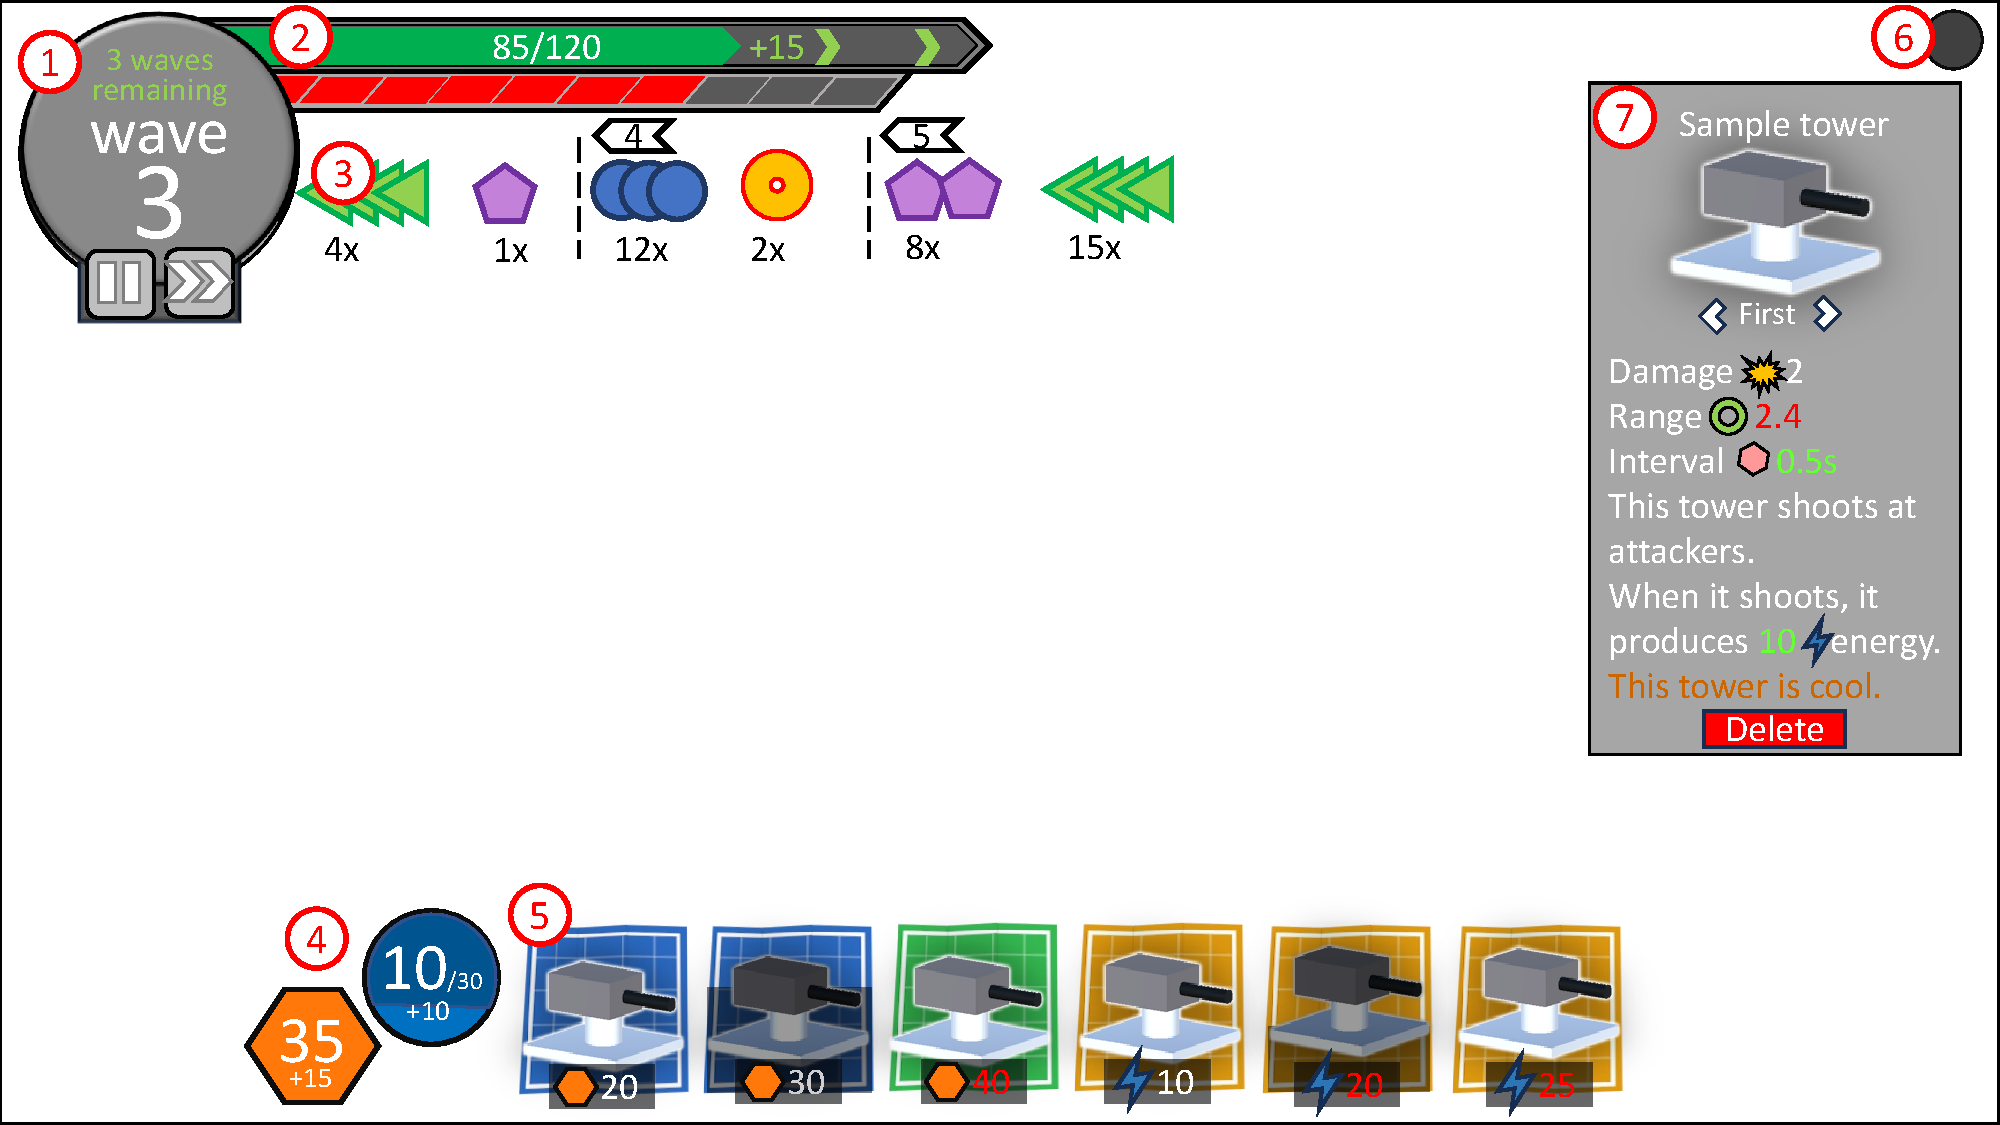
\includegraphics[width=\textwidth]{img/Battle UI design.pdf}
    \caption{A mockup of the GUI during a battle. Red numbers in circles marking the individual components.}
    \label{fig:battle-ui}
\end{center}

\subsection{Waves and time controls}

In the top left corner is displayed the number of the current wave in big white text.
Above it is the remaining number of waves in green.
This amount is calculated from the current amount of \emph{fuel} and the \emph{fuel} production per wave.

Below this, there is a panel with time controls.
Here, the player can start the next wave, or pause or speed up the game.
The pause button will change into play when the game is paused or between waves.
The speed button will change between one arrow and two arrows, based on the currently selected speed.

\subsection{Fuel and Hull}

Immediately to the right of the wave s display is displayed \emph{fuel} and \emph{hull}.
The green progress bar displays how much \emph{fuel} the player has out of the total required to finish the level.
It also displays these values in text.
Additionally, it shows the amount of \emph{fuel} produced per wave and light green marks previewing the \emph{fuel} values after each of the upcoming waves.

Below is a red progress bar showing the player's \emph{hull} out of the maximum amount.

\subsection{Wave Preview}

Below the \emph{fuel} and \emph{hull} displays it the wave preview.
It shows the composition of the current and upcoming waves.
Each wave has an arrow with its number and the batches of attackers that will come.
Each batch shows one or more icons of the attacker type it's composed of along with a count.
The icon spacing represents the spacing of the attackers in the wave itself.

\subsection{Materials and Energy}

At the bottom of the screen is the \emph{materials} and \emph{energy} display.
In the orange hexagon is shown the current amount of \emph{materials} the player has, along with a smaller number below it representing the \emph{material} production per wave.
Similarly, the blue circle shows the current amount of \emph{energy} and the \emph{energy} limit, with the \emph{energy} production below.
The circle is partially filled with a lighter blue to visually show how much \emph{energy} the player has out of the maximum.

\subsection{Blueprint Menu}

To the right of \emph{materials} and \emph{energy} is the blueprint menu.
Here the player can select their blueprints to use them.
Between waves, only buildings are shown, and during a wave, only abilities are shown.

Each blueprint is shown as a colored square of paper with an icon over it.
The color represents the type of the blueprint:
\begin{itemize}
    \item blue for towers,
    \item green for economic buildings,
    \item purple for special buildings
    \item and orange for abilities.
\end{itemize}
Overlaid over the lower portion of the blueprint is its cost.
This is what the blueprints look like everywhere in the game, for example in blueprint rewards.

The cost number turns red when the player has insufficient resources.
The cooldown is also shown as a partial dark transparent overlay over the blueprint paper.
The portion it covers represents the portion of the cooldown that's left until the blueprint can be used again.

By clicking on a blueprint in the blueprint menu, the player will select it.
To use it, they will have to click somewhere in the world to specify at which position do they want to use it.
The player will also be able to select the blueprints using the number keys \textbf{1} to \textbf{9} on their keyboard, based on the blueprint's position in the blueprint menu.

\subsection{Settings Button}

In the top right is a button which lets the player access a settings screen.
Here the player will be able to access some game settings like sound and music volume.
They will also be able to exit back to menu from this screen.
When the settings screen is opened during a wave, the game pauses.

\subsection{Info Panel}\label{sec:design-info-panel}

At the right edge of the screen is the info panel.
It shows up only when the player has selected something, and it displays information about the selected thing.
It also shows up when the player has not selected anything, but only hovered over something selectable with the cursor.
In this mode, the panel is semi-transparent and no buttons are showing (more information below).
This panel will appear whenever the player selects a relevant object, even on other screens, not just in battle.
For example, when the player selects a blueprint in a shop.

At the top is the name of the currently selected object.
For now, let's assume it's a tower, as shown in the picture.
The name is over a large icon of the tower's blueprint.

Over the lower portion of the icon is the targeting priority selector.
It is displayed only when there are targeting options to choose from.
Usually, only towers can have a targeting priority, and not all of them have it.
The targeting priority selector consists of the name of the currently selected priority, and arrows to the left and right of it to switch to the next or previous priority.
The priorities are usually a subset of those described in section~\ref{sec:design-towers}.

The main portion of the info box is taken up by the description.
The contents of the description depend on the selected object and will be specified later.
However, there is a few special features the description has that can appear no matter the selected object type.

First of them are icons in the text.
These icons are used for important stats or quantities that appear often.
For example there is an icon associated with damage, one for range, one for \emph{materials}, etc.
The icon usually appears before the mention of the thing it's associated with or before the stat.
Examples of this use can be seen in figure~\ref{fig:battle-ui}.

Most of the quantities in the description can be modified in various ways.
If there is some sort of original version which differs from the current version, we can highlight the changed quantities using colors.
Red means the quantity is now worse than before, green means it's better.
Note that for some statistics, higher is better, and for others, lower is better.
Additionally, it is possible something added a new description that wasn't in the original version.
For example, a special building could add new abilities to neighboring towers.
This new description is highlighted in orange.

Below the description is a button that allows the player to delete the selected building.
Of course, this button only appears when the selected object is a building that it is not permanent, unlike for example, the Hub.

As mentioned, the info panel will display the description of \textbf{blueprints}.
A blueprint's description contains sentences that explain what the thing, which the blueprint represents, does.
Additional quantities that don't fit into these sentences are summarized at the top, as shown in figure~\ref{fig:battle-ui}.
Also, when a blueprint is selected from the blueprint menu, it will show the remaining cooldown if any.

The descriptions of \textbf{buildings} are basically the same as their blueprints.
However, buildings can also provide some additional information of their own, for example the total amount of damage a tower has dealt or the amount of \emph{materials} a building has produced.

Similarly, \textbf{attacker stats} can be displayed, for example when you encounter a given attacker type for the first time.
The format is the very similar to blueprints with base stats (see section~\ref{sec:attacker-types}) at the top and additional abilities described in sentences below.
Attackers can also be selected during a wave.
The changes are the same as with buildings and blueprints, but also the attackers always show their current HP in addition to their max HP.

The player can also inspect an empty \textbf{tiles}.
Here only little information is provided.
Whether the tile has some obstacles, or is rich in \emph{minerals} or \emph{fuel}, whether it is slanted and whether a path runs across it.
If the tile has a building on it, the details of the building are displayed instead.

\section{Attacker HP Indicators}

During a wave, we want the attackers in the world to have HP indicators above them to communicate to the player how much more damage they need to deal to a given attacker to kill it.
These indicators should be overlaid over the attackers and always face the camera.
Their purpose is to let the player know how much HP the attacker has left.
There is going to be a lot of attackers on the screen, and thus a lot of HP indicators.
They should be simple in order to be legible when viewed when the camera is zoomed out and not too noisy in large quantities.

Thus, we will use the design displayed in figure~\ref{fig:attacker-hp}.
It has a rectangular shape, and it should be one size for all small attackers and one size for all large attackers.
The rectangle is filled in with a colored fill on a dark gray background.
This fill represents the portion of the attacker's HP that's left out of their maximum HP.

\begin{center}
    \captionsetup{type=figure}
    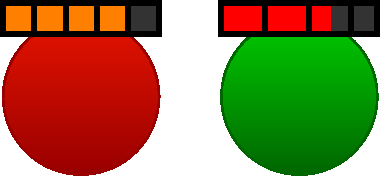
\includegraphics[width=0.5\textwidth]{img/Attacker HP.pdf}
    \caption{Two attackers with HP indicators. The one on the left has 4/5\,HP, the one on the right has about 150/250\,HP.}
    \label{fig:attacker-hp}
\end{center}

Over the colored fill, there are black vertical lines dividing the indicator into sections.
Each section represents the same amount of HP.
In the HP indicator above the attacker on the left, each section represents 1\,HP.
Thus, we can count that the attacker has 4\,HP out of a maximum of 5.
However, some attackers will have a lot of HP, and section of just 1\,HP would be impractical for those.
So each section will represent a power of~10 of HP, and we will distinguish them by the color of the fill.
Orange for 1\,HP sections, red for 10\,HP sections, dark red for 100\,HP sections, and potentially also magenta and purple if larger values are needed.

We always choose the largest section size that leads to the indicator having more than one section, so there is always 2 to 10 sections.
It is also important to note, that the rightmost section will not necessarily represent the amount of HP it should.
For example when an attacker has 250\,HP, their indicator will consist of two 100\,HP sections and one 50\,HP section.
This last section will be scaled accordingly, in this case it will be only half as wide as the whole sections, as seen in figure~\ref{fig:attacker-hp}.

\section{Selection and Highlighting}

In section~\ref{sec:design-info-panel} we've mentioned that the player will be able to select blueprints, buildings, tiles and attackers.
We want to communicate to the player what is currently selected.
We can accomplish this by displaying a blue outline around the selected object.
Similarly, we can show what's the player's cursor hovering over with a lighter shade of blue.

During a battle, buildings can often affect other objects, for example, towers usually have a big impact on the HP of surrounding attackers.
We can use similar highlights to show these relations.
All attackers within the range of a tower should be highlighted in yellow when that tower is selected.
Similarly, when placing an ability that immediately affects attackers, we should highlight the attackers that would be affected.
As another example, while the player is placing a building that affects other buildings, or when the player selects this building, all the affected buildings should be highlighted.
For some objects, for example most attackers, we don't even want to highlight anything else.
However, what to highlight will have to be decided on a case by case basis, because the objects in our game can have all sorts of unique behaviors.
Additionally, when the player hasn't selected anything, but has hovered over some object, we can also display its relevant highlights, since we're not displaying the highlights of any selected object.

Relevant objects won't be highlighted only based on what's selected.
As we indicated, when the player has selected a blueprint in order to use it, we can preview what would be affected if the player used it right now.
We should also highlight as hovered only the object relevant to the blueprint's placement.
When placing a building, we don't want to highlight the attacker the player's cursor is over, because building are not used on attackers.
They are built on tiles, so we should highlight the tile the attacker is on.
Similarly, when the player is about to use an ability that can be placed at any point on the surface of the world, we shouldn't highlight tiles or attackers, but only highlight the exact point the ability is about to be placed at.
This placement highlight can also indicate when a placement is invalid by turning red instead of being blue.

When placing something that can only be placed on specific tiles, we can also highlight these tiles.
For example, most towers cannot be placed on tiles with obstacles or a path.
There is usually going to be a lot of valid tiles, so this highlight should be a bit more subtle.
We think the best way to show this is to tint the terrain of the valid tiles in blue.

We also want to show the range of the ability or tower the player is currently placing (or a tower that's selected).
The player needs to see the range in the context of the world, just a number is not enough.
The most clear way to do this is to also draw this range visualization directly on the terrain.
This is because the situation could be viewed from different angles.
In most cases, this would be just a simple circle, however, some towers or abilities can have an unusual range shape, for example a straight line.
Most importantly, a lot of towers will only be able to shoot at attackers in line of sight, which will create all sorts of unusual range shapes.
We definitely need to communicate to the player where the tower can hit attackers and where it cannot.

In figure~\ref{fig:range-visualization} is an example range visualization for a tower that requires line of sight.
This situation is showed from a top-down view, however in game, this would take place on a 3D terrain and this range visualization would have to be drawn correctly even from a different angle.
In the figure, the tower is represented by the blue square in the center.
The black lines separate different levels of the terrain, the lowest level is colored with the darkest shade of gray.
In the top part of the figure, we can see the tower's line of sight is being blocked by a higher terrain.
The visualization also shows that this tower cannot shoot uphill, since there is nothing drawn on the higher level of the terrain.
In the top left quadrant we can see the tower's line of sight by some large obstacles.
The tile immediately to the right of the tower is slanted, transitioning to a lower level.
On the lower level, we can see some unusual shapes emerge.
This gap in the range appears, because the terrain level the tower is on is in the way when the tower wants to shoot at attackers close to the base of the overhang.

\begin{center}
    \captionsetup{type=figure}
    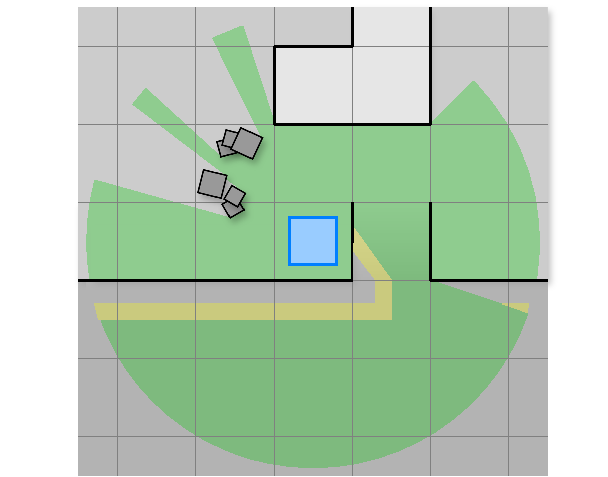
\includegraphics[width=0.9\textwidth]{img/Range visualisation.pdf}
    \caption{Example visualization of the range of a tower represented by the blue square.}
    \label{fig:range-visualization}
\end{center}

Here, we can also see a portion of the range colored in yellow.
This means that if an attacker was at this point, the tower would only be able to shoot at it over the ledge if it was a \emph{large} attacker.
In section~\ref{sec:attacker-types} we have explained that there will be two sizes of attackers.
This means that there will be a region where a tower can't see any attackers, a region where the tower can see any attackers (green), a region where the tower can only see \emph{large} attackers (yellow), but also a region where the tower can only see \emph{small} attackers.
The last case is, however, very rare, so we can draw this region also in green.

Calculating the exact shape of the region the tower can see can be expensive.
We could simplify this by only computing the range visualization where an attacker could appear~--- on a path.
However, we think it is important to show at least an approximation of the whole picture, to make it easier for the player to see what's blocking the line of sight and where.

\section{Battle Camera Controls}

During a battle, the world will be rendered onto the player's screen using an orthographic camera at an angle that mimics isometric graphics~\cite{IsometricWiki}.
The world is pretty large, so we want to let the player zoom in.
They will be able to do so using the mouse scroll wheel.
Most of the time, the world will be viewed at an angle in to clearly convey the various heights of the 3D terrain.
However, in some cases it would be useful to have a top-down view, for example when inspecting whether a path intersects with a tower's range.
We can blend these functions by slowly tilting the camera to look straight down at the maximum zoom level.
This is the zoom level at which it's best to inspect details anyway.

Since the camera can be zoomed in, the whole world won't necessarily be on the screen at once.
The player will have to be able to move the camera around.
Additionally, high terrain can sometimes obstruct what's behind it, so we will allow the player to rotate the camera around the vertical axis, bot only in 90~degree steps to preserve the isometric look.

\section{Future Features}

In this section, we would like to mention other features that will be in the full game, and we've not described them earlier in this chapter.
These features will also have to be designed eventually, but they will not be in the demo, so only rough descriptions are provided.

\begin{notindemo}

    \subsection{Setting and Story}

    From the names we've given to various game components, it might be clear that we're leaning towards some kind of sci-fi setting.
    The player would travel across a galaxy using a spaceship, stopping on various planets along the way to refuel for further travels.
    But what is the main character's story?
    What is their ultimate goal?
    Well, the story has not been decided yet.
    However, the story should be an important part of the game, and it will inform a big portion of the game's further design.
    Any game can always benefit from an engaging story, especially single-player games.

    \subsection{Run Structure}

    We want each run of the game to last at most 2~hours, since we want the players to be able to complete each run in on sitting.
    Each run will probably consist of three acts, each ending in a boss level.
    This is the same structure as in \emph{Slay the Spire} or \emph{Monster Train}~\cite{MonsterTrain}, which are both roguelike deck-building games.
    It seems to work very well for them, so it is where we'll start.
    However, the final run structure will heavily depend on playtesting.

    One thing that is clear even now, is that each battle will take substantially longer than in \emph{Slay the Spire}.
    \emph{Monster Train} also has longer levels, so each run consists only of 9~fights.
    It is reassuring to know that a roguelike of this kind can work even with fewer levels.
    Even though \emph{Monster Train} has fewer levels than \emph{Slay the Spire}, it has a similar amount of rewards and shops throughout the run, letting the players customize their build to a similar degree, if not greater.

    \subsection{Saving the Game}\label{sec:design-saving}

    Even though we want the players to be able to play a run in one sitting, saving their progress is still a very useful feature.

    Ideally, we would save the game after every choice the player makes and after every tick of simulation during a battle.
    However, this is technically unfeasible.
    We could save the game whenever they explicitly choose to save, for example when they exit the game.
    This would still be pretty difficult, since we would need to serialize the state of all towers, attackers and projectiles, and then we would need to be able to load and initialize everything correctly again.

    We could take the approach both \emph{Slay the Spire} and \emph{Monster Train} use and save the game whenever the player makes a decision outside of battle, and during battle only at the start and the end.
    This would definitely work and be usable.
    However, we will aim to save the game at the start and end of every wave.
    In \emph{Bloons TD 6}, the game is saved at the end of every wave only, and the player can build towers even during a wave.
    This means that a player can exit the game right before they would lose and redo the wave, with a different strategy.
    In our game this sort of save scumming would be less effective, since during a wave, the player can only use abilities, which are meant to be used reactively anyway.

    \subsection{Money}

    We that it would be good to add another resource, one that persists throughout the entire run.
    The main use of this resource, for simplicity called money, would be to pay for items in shops.
    This would allow the player to make more decisions than for example, if they got one thing in every shop for free and nothing more.
    This way they can save up their money when a shop doesn't offer anything they'd like to buy, and spend more at shops with things they like.
    Of course, money would be acquired mainly by winning battles and sometimes in events.

    \subsection{Permanent Unlocks}

    The most strict definitions of a \emph{rogue-like} mandate that the game doesn't let the player unlock any permanent improvements which persist between runs.
    The players themselves should improve by playing the game, not their in-game characters.
    We like this idea and wish to preserve it even within our game.
    However, it is possible the player will be able to unlock more of our game's content as they play, in a way that is similar to \emph{Slay the Spire}.
    In \emph{Slay the Spire}, the player starts off as a character called \emph{The Ironclad} and only after playing one game they unlock the second character.
    Furthermore, for each character, the game offers five sets of new cards and relics to unlock.
    These unlock serve mainly to not overwhelm a new player with choices or items which are harder to understand.

\end{notindemo}